In this chapter, we present the results following the methodology described in Chapter~\ref{chapter:methodology}. We first present the results of the data exploration, preprocessing and augmentation. We then present the results of the automated evaluation, including topic coherence scores, topic diversity scores, silhouette scores, comparison with baseline models, and hyperparameter tuning. Then, we show the tag generation pipeline, including the base BERTopic model and its subcomponents and hyperparameters, the additional fine-tuning model, and zeroshot classifier. Finally, we present the results of the human evaluation, followed by the results of the large-scale automated evaluation.

\section{Data exploration, preprocessing and augmentation}
\label{sec:data_exploration}
Following an initial exploratory data analysis, we identified several methods for augmenting the dataset descriptions. The dataset descriptions are augmented with the following additional information:

\begin{itemize}
    \item \textbf{Name} — The name of the dataset.
    \item \textbf{Tags} — The generated tags that have already been created for the dataset.
    \item \textbf{Features} — The names of the dataset's features (columns).
    \item \textbf{Scraped text} — For some datasets, we scrape text from the original sources and append it to the dataset description.
\end{itemize}

Additionally, we remove all datasets that have a cosine similarity of 0.99 or higher with another dataset, as these datasets are likely to be duplicates or different versions of the same dataset. This results in the removal of $\sim$300 datasets from the original $\sim$5500 datasets.

After augmenting the dataset descriptions, we observe that the augmented descriptions are longer, and potentially more informative, as illustrated in \cref{fig:description_vs_augmented_description}. All subsequent analyses are performed on the augmented dataset descriptions.

\begin{figure}[h]
    \centering
    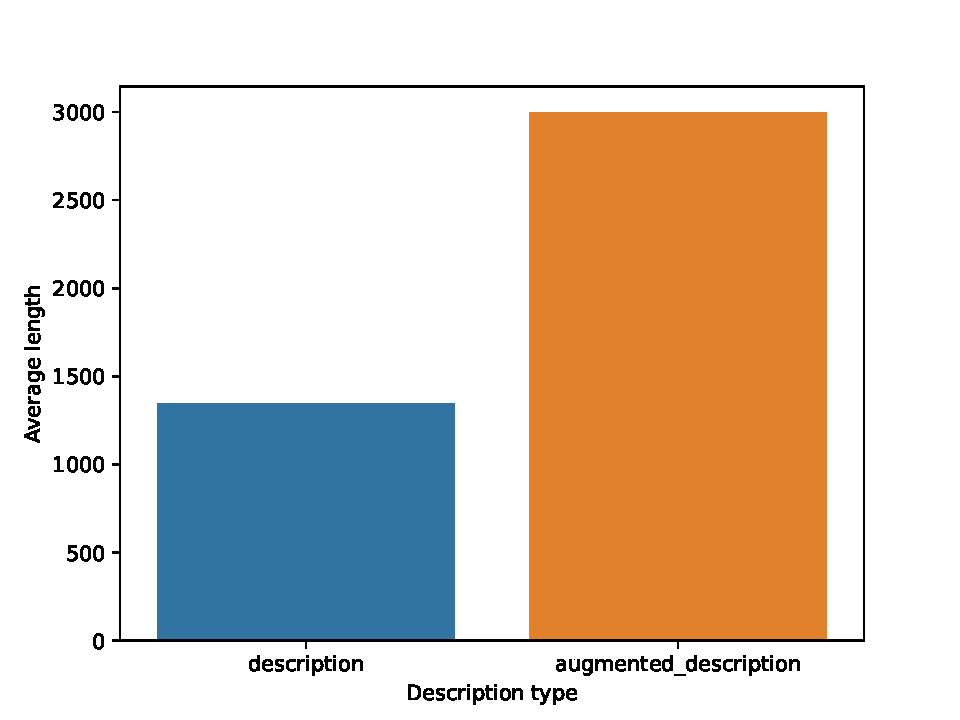
\includegraphics[width=0.65\textwidth]{figures/description_vs_augmented_description.pdf}
    \caption{Histogram of the length of dataset descriptions vs augmented dataset descriptions}
    \label{fig:description_vs_augmented_description}
\end{figure}

\cref{fig:length_of_descriptions} presents a histogram depicting the length of dataset descriptions. The lengths range from 0 to 10,000 words, with the majority of descriptions being under 5,000 words. A few outliers exceed 10,000 words.

\begin{figure}[h]
    \centering
    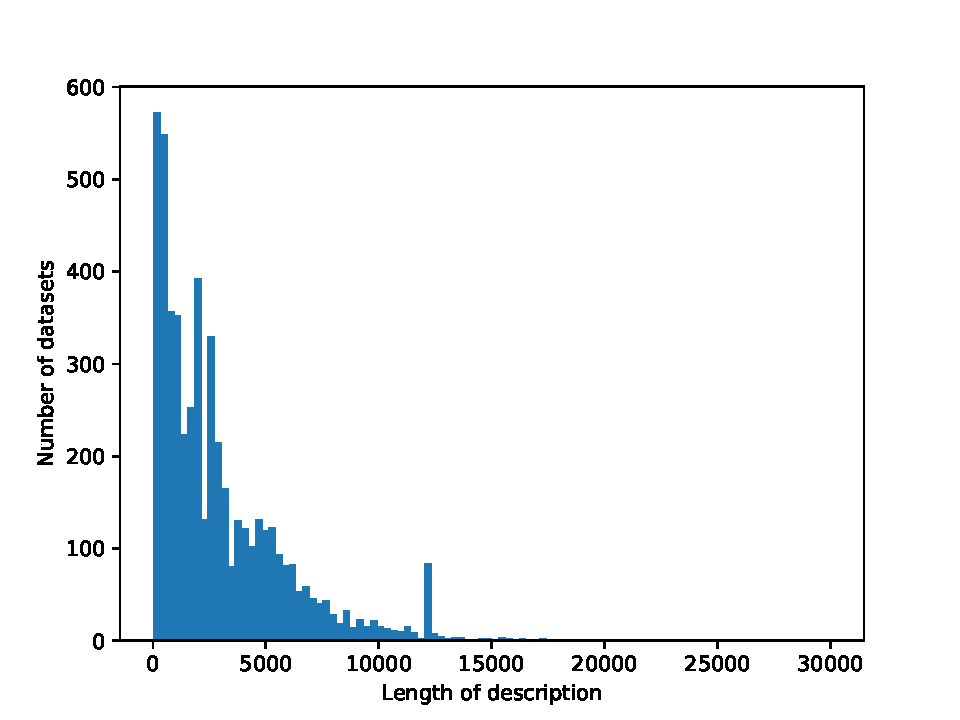
\includegraphics[width=0.85\textwidth]{figures/length_of_descriptions.pdf}
    \caption{Histogram of the length of dataset descriptions}
    \label{fig:length_of_descriptions}
\end{figure}

Similarly, \cref{fig:words_of_descriptions} and \cref{fig:sentences_of_descriptions} display comparable distributions, this time for the number of words and the number of sentences, respectively.

\begin{figure}[h]
    \centering
    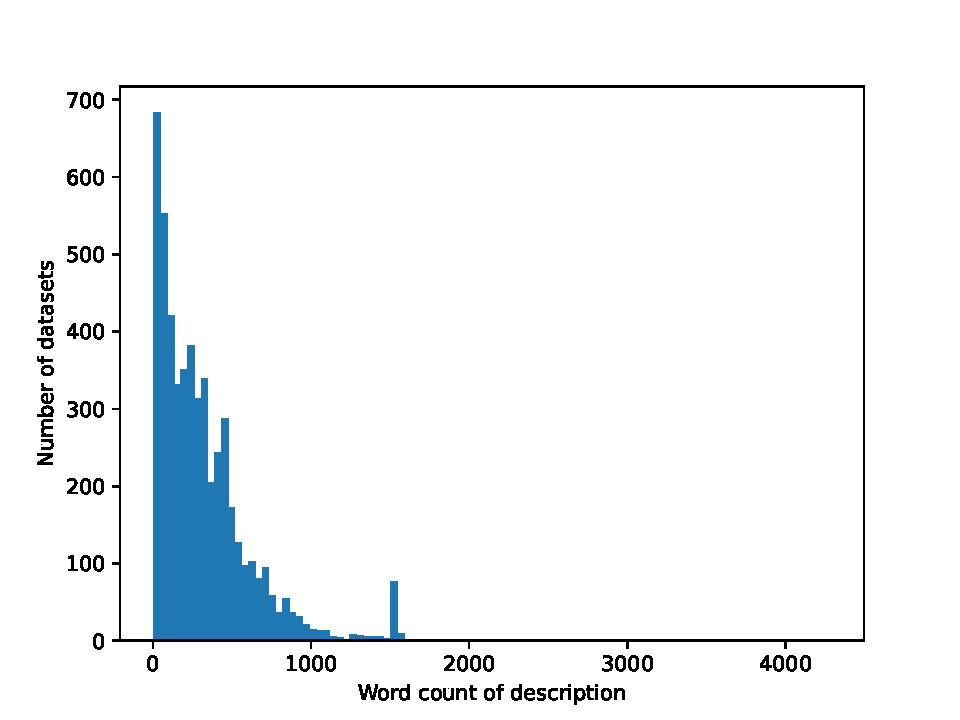
\includegraphics[width=0.85\textwidth]{figures/words_of_descriptions.pdf}
    \caption{Histogram of the number of words of dataset descriptions}
    \label{fig:words_of_descriptions}
\end{figure}

\begin{figure}[h]
    \centering
    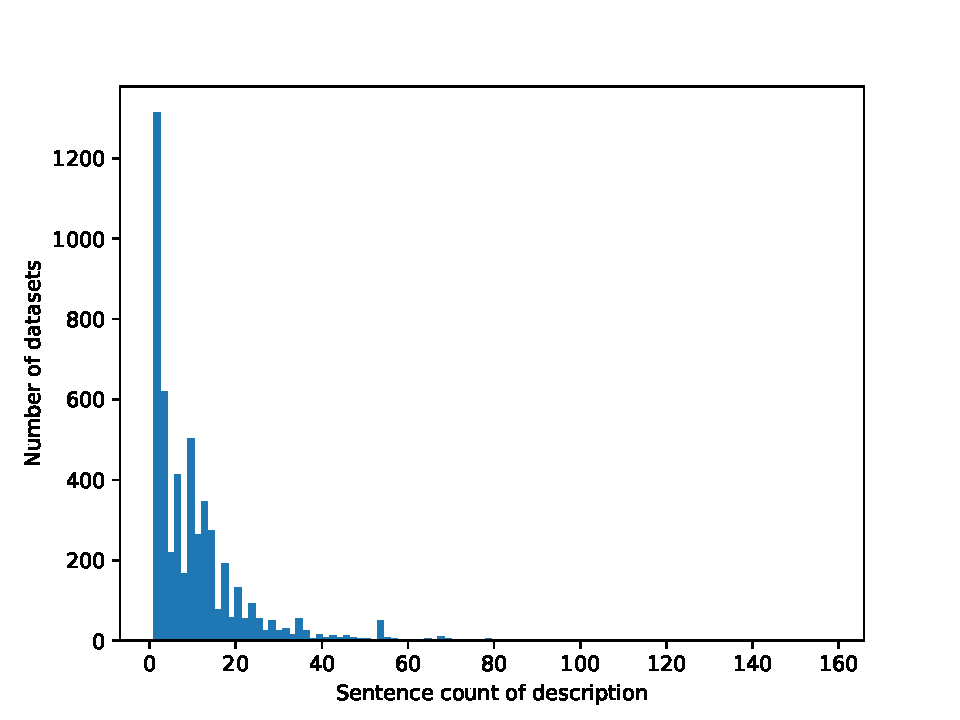
\includegraphics[width=0.85\textwidth]{figures/sentences_of_descriptions.pdf}
    \caption{Histogram of the number of sentences of dataset descriptions}
    \label{fig:sentences_of_descriptions}
\end{figure}

When we examine the availability of tags, we find that the majority of datasets already have tags associated with them (\cref{fig:tag_availability}). This suggests that the tag generation model may be able to leverage the existing tags to improve its performance.

\begin{figure}[h]
    \centering
    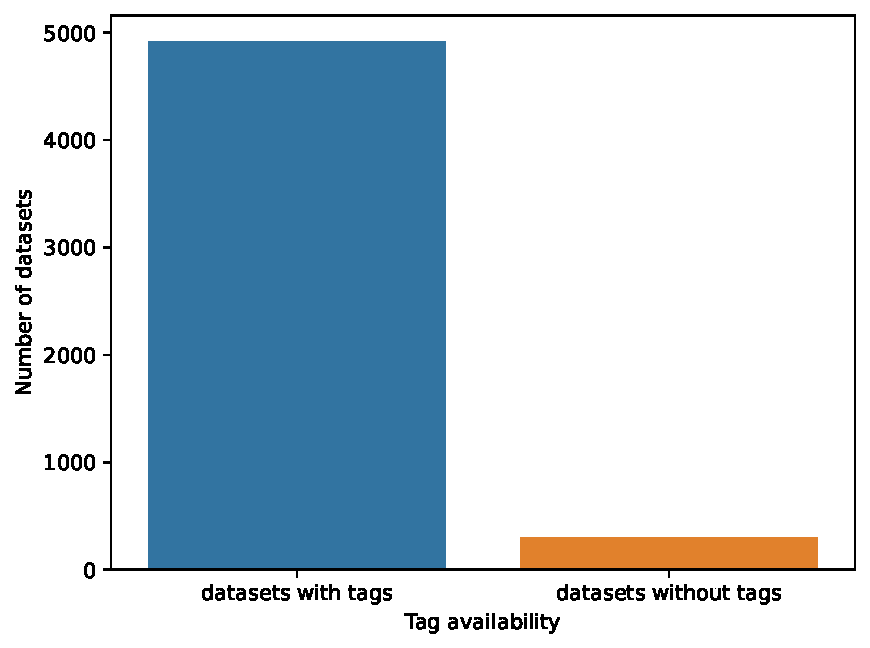
\includegraphics[width=0.85\textwidth]{figures/tag_availability.pdf}
    \caption{Histogram of the number of datasets with and without tags}
    \label{fig:tag_availability}
\end{figure}

When we analyze the number of tags associated with each dataset, we find that most datasets have between 0 and 5 tags, with a few datasets having more than 5 tags (\cref{fig:number_of_tags}).

\begin{figure}[h]
    \centering
    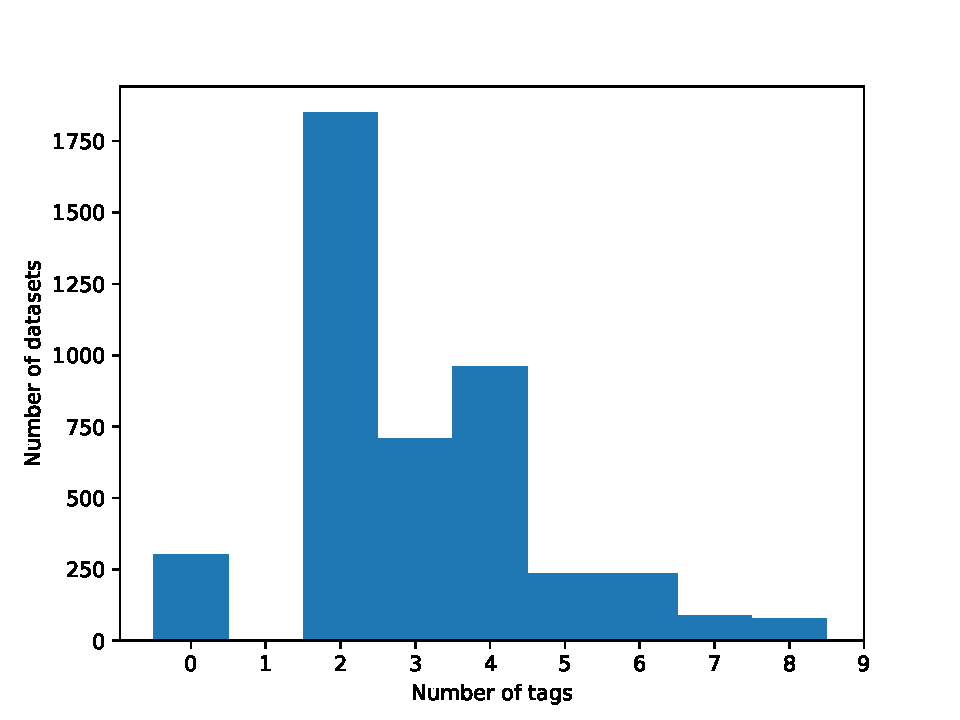
\includegraphics[width=0.85\textwidth]{figures/number_of_tags.pdf}
    \caption{Histogram of the number of tags associated with datasets}
    \label{fig:number_of_tags}
\end{figure}

We then look at the number of features (columns) in the datasets. The distribution of the number of features is shown in \cref{fig:number_of_features}. Most datasets have fewer than 100 features, with a large number of datasets having more than 100 features. This is because those datasets are likely to be high-dimensional datasets from domains such as genomics, text processing, or image analysis, where numerous variables or measurements are collected for each sample.

\begin{figure}[h]
    \centering
    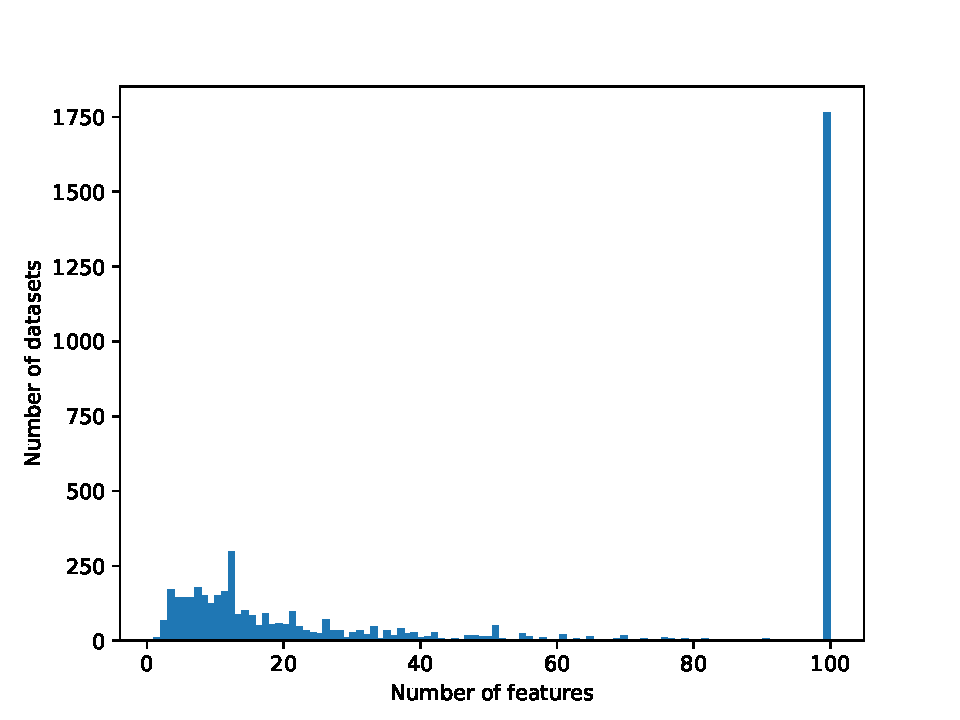
\includegraphics[width=0.7\textwidth]{figures/number_of_features.pdf}
    \caption{Histogram of the number of features in datasets}
    \label{fig:number_of_features}
\end{figure}

Additionally, we examine the cosine similarity between the augmented dataset descriptions to see whether there are datasets with similar descriptions and duplicates. The heatmap of the cosine similarity is shown in \cref{fig:cosine_similarity}. The majority of dataset descriptions have a low cosine similarity, indicating that they are distinct from one another. However, there are some datasets with high cosine similarity, suggesting that they may be duplicates or different versions of the same dataset.

\begin{figure}[h]
    \centering
    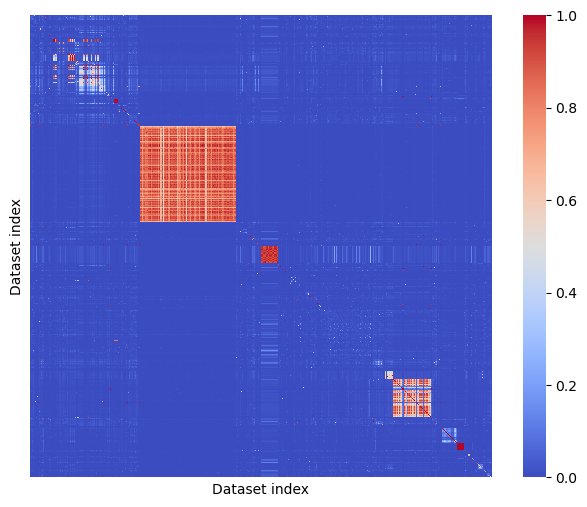
\includegraphics[width=0.85\textwidth]{figures/cosine_similarity.png}
    \caption{Heatmap of the cosine similarity between dataset descriptions}
    \label{fig:cosine_similarity}
\end{figure}

We find that OpenML datasets can have multiple versions. Our analysis of dataset versions reveals that most datasets have only 2 versions, though several datasets have more than 2 (\cref{fig:number_of_versions}).

\begin{figure}[h]
    \centering
    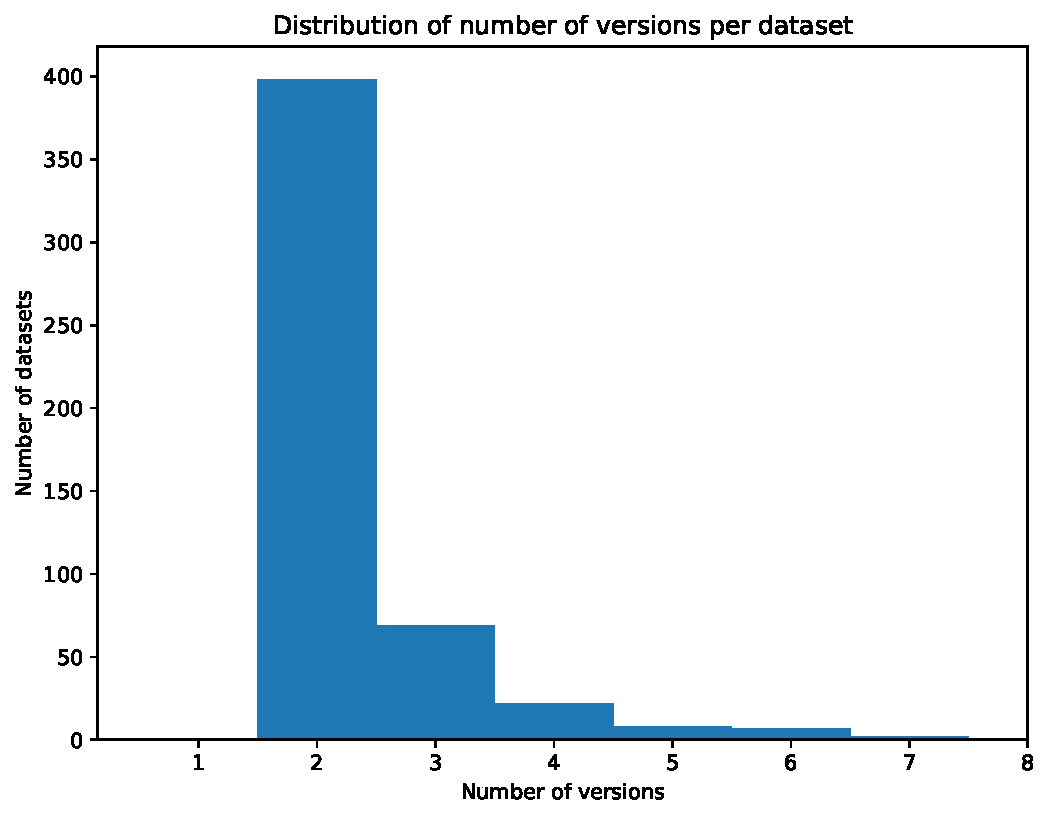
\includegraphics[width=\textwidth]{figures/number_of_versions.pdf}
    \caption{Histogram of the number of versions of dataset descriptions}
    \label{fig:number_of_versions}
\end{figure}

We also examine the similarity between different versions of the datasets. Our analysis shows that most datasets have a cosine similarity of 0.9 or higher within versions, suggesting that the versions are highly similar to one another (\cref{fig:cosine_similarity_dataset_versions}).

\begin{figure}[h]
    \centering
    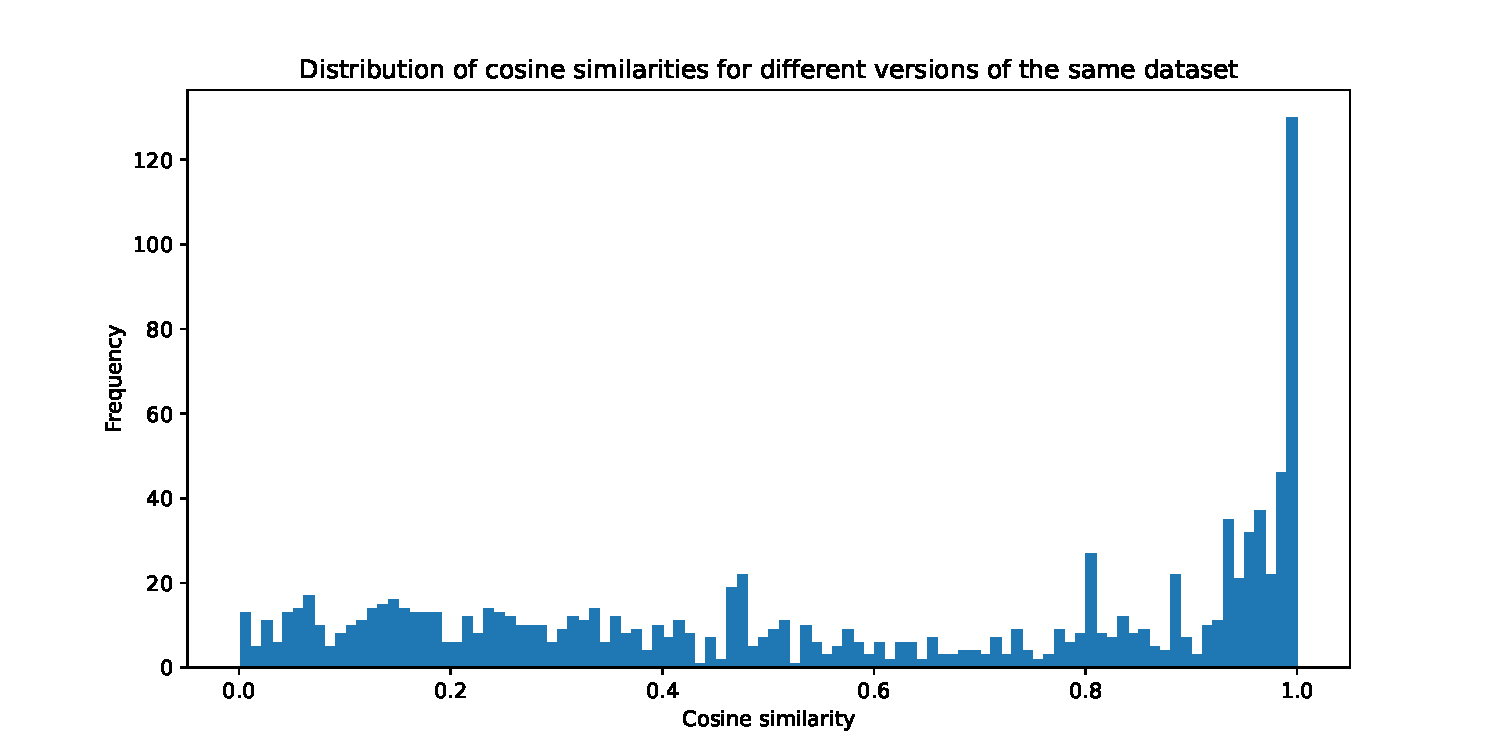
\includegraphics[width=\textwidth]{figures/cosine_similarity_dataset_versions.pdf}
    \caption{Histogram of the cosine similarity of different versions of dataset descriptions}
    \label{fig:cosine_similarity_dataset_versions}
\end{figure}

From these histograms, we can infer that the dataset descriptions are relatively short, with the majority being comparable in length to two Twitter tweets. This is important to note, as descriptions that are too short may lack enough information to generate meaningful tags. However, this may not necessarily pose an issue, as prior studies have successfully applied topic modeling to tweets and other short texts \cite{cataldi_emerging_2010, churchill_percolation-based_2020, curiskis_evaluation_2020, kasiviswanathan_emerging_2011, paul_discovering_2014, yin_dirichlet_2014}.

We applied Named Entity Recognition (NER) and Part-of-Speech (POS) tagging to the dataset descriptions to identify the most common entities and parts of speech (\cref{fig:pos,fig:ner}). A significant number of words were tagged as \textit{X}, indicating that the POS tagger was unable to determine the part of speech for these words. This is likely due to the presence of domain-specific terms not included in the POS tagger's vocabulary, as well as unrecognized or anomalous tokens and symbols. Additionally, we found that the most frequent named entity is \textit{PERSON}, which can be attributed to the fact that many dataset descriptions reference the names of dataset authors or associated papers. Both of these findings pose challenges for the performance of the tag generation model, as unrecognized tokens and author names do not contribute meaningful information for generating relevant tags.

\begin{figure}[h]
    \centering
    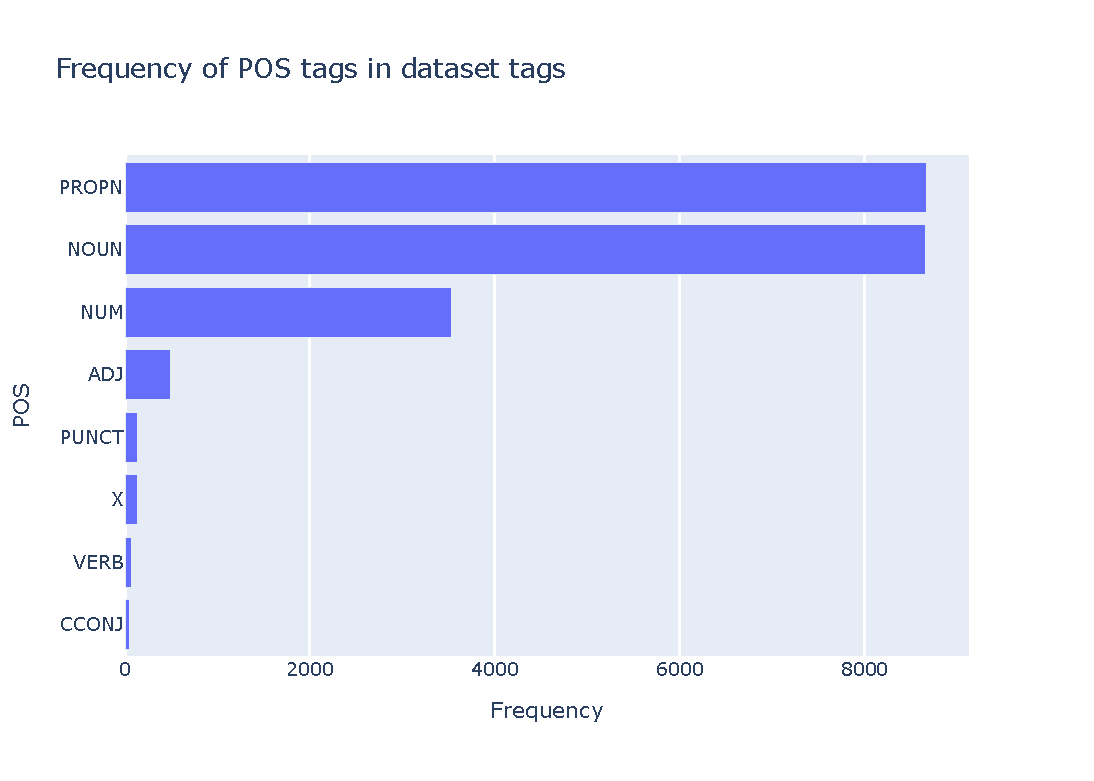
\includegraphics[width=0.9\textwidth]{figures/pos.pdf}
    \caption{Bar chart of the most common parts of speech in dataset descriptions}
    \label{fig:pos}
\end{figure}

\begin{figure}[h]
    \centering
    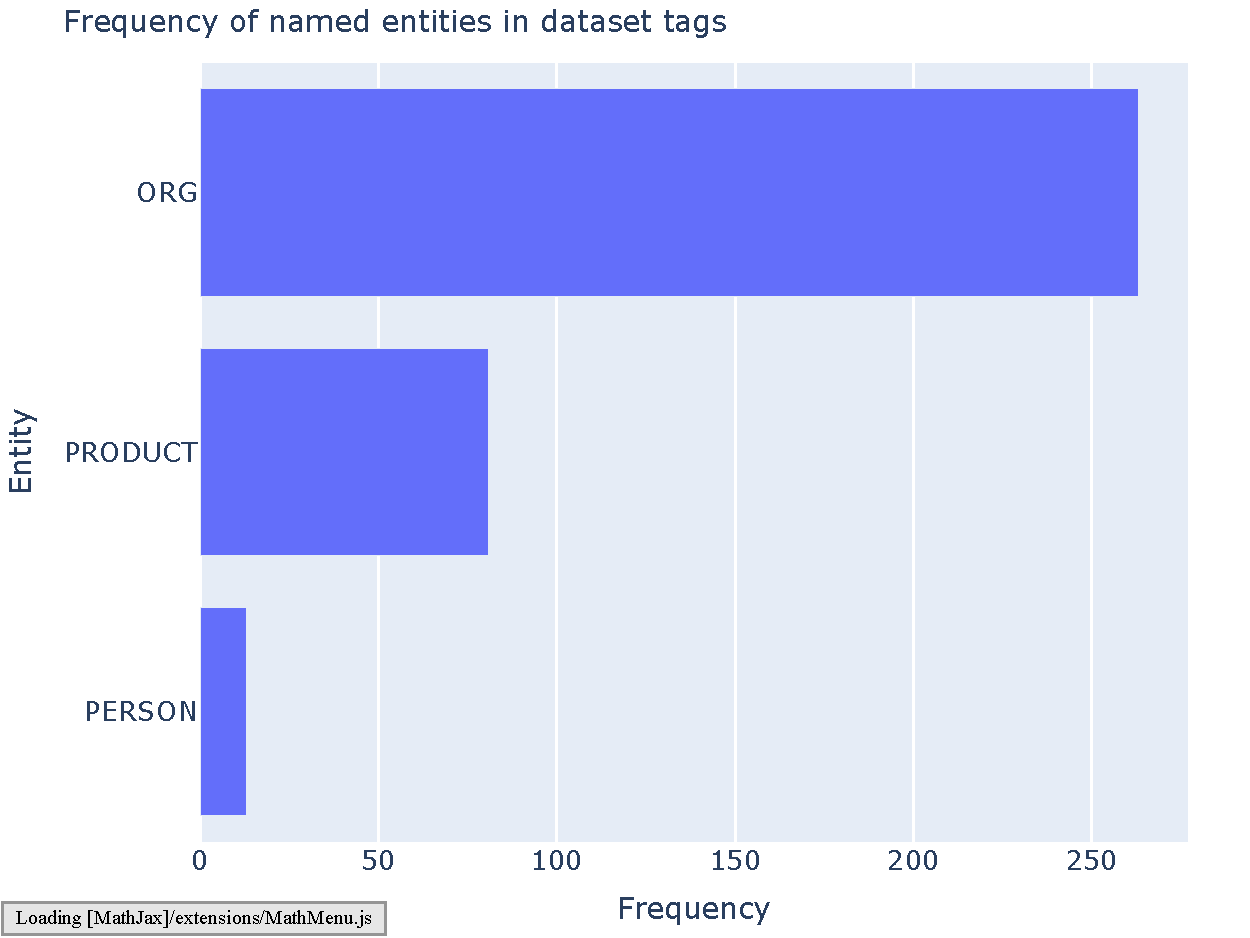
\includegraphics[width=0.9\textwidth]{figures/ner.pdf}
    \caption{Bar chart of the most common named entities in dataset descriptions}
    \label{fig:ner}
\end{figure}

We also examine how many datasets include URLs to original sources in their descriptions (\cref{fig:url_availability}). A significant number of datasets contain URLs, which could be used to scrape additional text for augmenting the descriptions. However, upon closer inspection, we find that the information in these URLs is often redundant with what is already provided in the dataset descriptions. Nonetheless, for some datasets, the URLs contain supplementary information that could be valuable for generating tags, which we then scrape.

\begin{figure}[h]
    \centering
    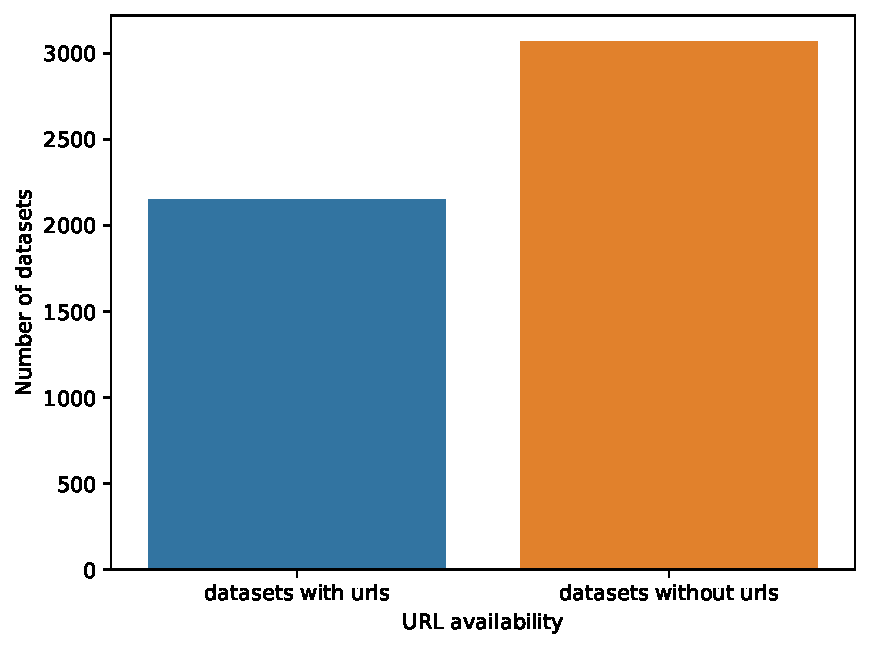
\includegraphics[width=0.85\textwidth]{figures/url_availability.pdf}
    \caption{Bar chart of the number of datasets with and without URLs to original sources}
    \label{fig:url_availability}
\end{figure}

We also explore the readability and complexity of the dataset descriptions by calculating the Flesch Reading Ease \cite{flesch_new_1948} (\cref{fig:flesch_reading_ease}). The Flesch Reading Ease score ranges from 0 to 100, with higher scores indicating easier readability. We find that the dataset descriptions are somewhat difficult to read, with many falling in the 0-60 range. This suggests that the descriptions may contain complex language and jargon that could require specialized knowledge to understand. This may also affect the embedding model performance, as it may struggle to capture the semantic meaning of complex or domain-specific terms which the embedding model has not been trained on.

\begin{figure}[h]
    \centering
    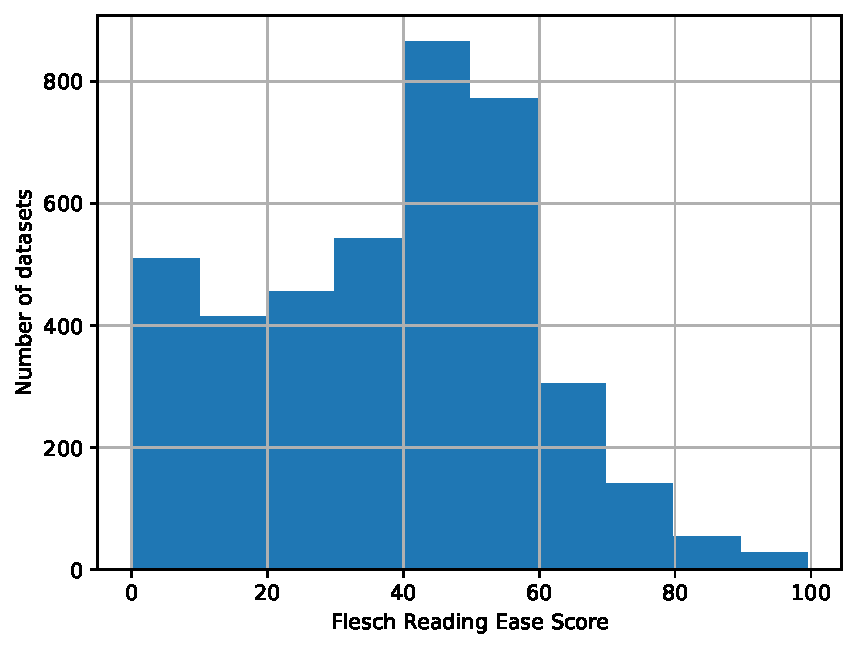
\includegraphics[width=0.85\textwidth]{figures/flesch_reading_ease.pdf}
    \caption{Bar chart of the number of datasets with and without URLs to original sources}
    \label{fig:flesch_reading_ease}
\end{figure}

In this section, we described the most pertinent findings from our data exploration. For readers interested in a more detailed analysis, additional information can be found in the \textit{eda.ipynb} notebook in the \href{https://github.com/ivangermanov/openml-tags}{GitHub repository} \cite{germanov_topic_modeling_of_2024}.

\section{Automated evaluation metrics and baselines}
We first explain the hyperparameter tuning (Bayesian optimization) process. Then, we explain the baseline models we use and what parameters we choose for them. We showcase the results of the comparison between the baseline models and the hyperparameter-optimized BERTopic model.

\subsection{Hyperparameter tuning}
Using OCTIS, we perform hyperparameter tuning for a BERTopic model. As an objective metric, we use the weighted metric we defined in \cref{sec:hyperparameter_tuning}. We set ranges for the hyperparameters, which are based on prior knowledge of good default values and the OpenML dataset characteristics. The hyperparameters and their respective search spaces are as follows:

\begin{itemize}
    \item \textbf{min\_topic\_size}: This determines the minimum number of documents a topic should have. We set the range to [2, 3] to explore small topic sizes.
    \item \textbf{ctfidf\_reduce\_frequent\_words}: This boolean hyperparameter determines whether frequent words should be reduced when constructing the c-TF-IDF matrix. The values considered are \texttt{True} or \texttt{False}.
    \item \textbf{umap\_n\_neighbors}: This hyperparameter controls the number of neighbors considered in the UMAP algorithm. We set the range to [2, 3]. We choose smaller values, since larger values result in more global views of the manifold, while smaller values result in more local data being preserved.
    \item \textbf{umap\_n\_components}: This controls the number of dimensions UMAP reduces the embeddings to. We have set the range to [2, 10].
    \item \textbf{umap\_min\_dist}: This defines the minimum distance between points in the UMAP embedding space. We are exploring a small range of [0.0, 0.01].
    \item \textbf{umap\_metric}: The metric used to calculate distances between points in the UMAP algorithm. The two metrics we consider are 'cosine' and 'euclidean'.
    \item \textbf{hdbscan\_min\_cluster\_size}: This defines the minimum cluster size for HDBSCAN. We set the range to [2, 3]. Similarly to \texttt{min\_topic\_size} and \texttt{umap\_n\_neighbors}, we explore small values to capture smaller clusters.
    \item \textbf{hdbscan\_metric}: This defines the distance metric used by HDBSCAN. We restrict this to 'euclidean'.
    \item \textbf{hdbscan\_cluster\_selection\_method}: This determines how clusters are selected in HDBSCAN. We use 'eom' (excess of mass).
    \item \textbf{vectorizer\_ngram\_range}: This defines the n-gram range for the vectorizer. We consider both unigram (1,1) and bigram (1,2) settings.
    \item \textbf{vectorizer\_stop\_words}: We set the stop words for vectorization to be 'english'.
    \item \textbf{vectorizer\_tokenizer}: This boolean hyperparameter controls whether a custom tokenizer is used. We set this to \texttt{False}.
    \item \textbf{outliers\_strategy}: This defines how outliers should be handled. For this study, we set it to 'none', meaning that no specific outlier handling strategy is applied.
    \item \textbf{embedding\_model}: This hyperparameter defines the embedding model used for the BERTopic model. Since they are slower to evaluate, we only consider the \texttt{Salesforce/\allowbreak SFR-Embedding-\allowbreak Mistral} model, as it was SOTA on the MTEB leaderboard at the time of writing.
    \item \textbf{representation\_model}: This hyperparameter defines the representation model used for the BERTopic model. Since they are slower to evaluate, we only consider spaCy's Part-of-Speech model called \texttt{en\_core\_web\_lg}.
\end{itemize}

This automated hyperparameter optimization process allows us to systematically explore the space of possible configurations and identify the best-performing model for our dataset.

As for the Bayesian optimization \cite{archetti_bayesian_2019, galuzzi_hyperparameter_2020, snoek_practical_2012}, we employ the \texttt{Optimizer} class from OCTIS. This method efficiently explores the hyperparameter space by constructing a probabilistic (surrogate) model to approximate the objective function. In our case, the surrogate model is a Random Forest (RF), which is updated iteratively to predict the performance of unobserved hyperparameter configurations based on previous evaluations.

The surrogate model relies on the Matern kernel with a smoothness parameter \( \nu = 1.5 \). This kernel helps balance the trade-off between exploration and exploitation by controlling the smoothness of the Gaussian process used in the optimization.

To guide the search for optimal hyperparameters, we use the Lower Confidence Bound (LCB) acquisition function. The LCB acquisition function is particularly effective in encouraging exploration of uncertain regions while still exploiting areas that show high potential for improvement.

Before the optimization begins, we initialize the surrogate model with a diverse set of hyperparameter configurations. These initial points are generated using Latin Hypercube Sampling (LHS), which ensures a broad coverage of the search space from the outset.

Additionally, we set the number of iterations for the optimization process to 125, and the number of model runs per iteration to 3. This configuration allows us to explore the hyperparameter space thoroughly while maintaining a reasonable computational cost. We set the model runs to 3 to account for the stochastic nature of the BERTopic model (specifically, UMAP), which can yield slightly different results for each run.

\cref{fig:bayesian_optimization} shows the results of the Bayesian optimization process. The x-axis represents the number of iterations, while the y-axis represents the weighted metric score, \textit{Median(model\_runs)} and \textit{Mean(model\_runs)}, and other metrics. We can see that the optimization process converges to a stable solution relatively quickly. This indicates that the hyperparameter search space has been thoroughly explored, and a good configuration has been found.

\begin{figure}[h]
    \centering
    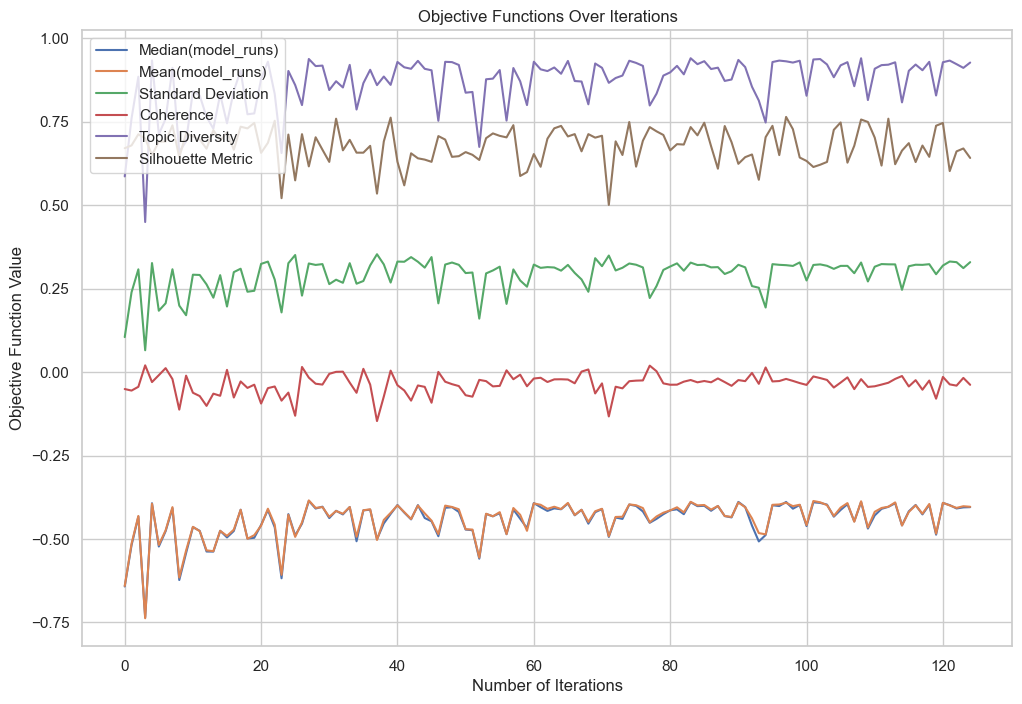
\includegraphics[width=0.8\textwidth]{figures/bayesian_optimization.png}
    \caption{Results of the Bayesian optimization process}
    \label{fig:bayesian_optimization}
\end{figure}

\subsection{Baselines}
\subsubsection{Definition of Baselines}
We select the hyperparameter-optimized BERTopic model as our primary model and compare its performance against several baseline models. The baseline models are as follows:
\begin{enumerate}
    \item \textbf{BERTopic model with default parameters}: This model uses the default hyperparameters provided by the BERTopic library. We use this model to compare the performance of the hyperparameter-optimized model with the default settings.
    \item \textbf{LDA}: We fit an LDA model to the dataset descriptions using the \texttt{LDA} class from OCTIS. LDA is a model which requires cleaning and preprocessing of the text data, such as removing stop words, stemming, and lemmatization. We use the default settings for the LDA model.
    \item \textbf{NMF}: We fit an NMF model to the dataset descriptions using the \texttt{NMF} class from OCTIS. We use the default settings for the NMF model.
    \item \textbf{CTM}: We fit a CTM model to the dataset descriptions using the \texttt{CTM} class from the Contextualized Topic Models library \cite{noauthor_milanlproccontextualized-topic-models_2024}. We preprocess the data and create the required embeddings with the \texttt{all-mpnet-base-v2} embedding model and use the default settings for the CTM model with the \texttt{contextual\_size} parameter set to 768.
    \item \textbf{Top2Vec}: We fit a custom implementation of Top2Vec based on the original model. This implementation uses the \texttt{all-mpnet-base-v2} embedding model from the Sentence Transformers library for document and word embeddings. The HDBSCAN clustering algorithm is used with custom arguments set in the \texttt{hdbscan\_args} parameter. We use the \texttt{Top2VecNew} class from our custom implementation, which allows for more flexibility in topic number specification.
\end{enumerate}

For each model, we train using a predefined set of topic numbers. This approach is necessary because some models require a fixed number of topics, while others, such as BERTopic, can either operate with a fixed number or determine the number of topics automatically. Specifically, we set the number of topics to 10, 20, 30, 40, 50, 100, and 200.

Additionally, for each specified number of topics, we run each model 10 times to account for their stochastic nature. This approach allows us to later assess whether there are statistically significant differences in the models' performance.

\subsubsection{Results}
In \cref{fig:openml_npmi} we present the NPMI scores for the hyperparameter-optimized BERTopic model and the baseline models. The NPMI score is a measure of topic coherence, with higher scores indicating more coherent topics. There are several BERTopic models with different hyperparameters:
\begin{itemize}
    \item \textbf{BERTopic\_optimized\_POS\_reduced\_range}: The BERTopic model we optimized with Bayesian optimization above.
    \item \textbf{BERTopic\_optimized\_POS\_full\_range}: Similar to the previous model, but with a wider range of hyperparameters. We choose not to use this model as we are interested in exploring smaller topic sizes, but we provide it for comparison.
    \item \textbf{BERTopic\_POS}: The BERTopic model with default hyperparameters (also with the spaCy Part-of-Speech model as the representation model).
    \item \textbf{BERTopic\_POS\_mpnet}: Similar to the previous model, but with the \texttt{all-mpnet-base-v2} embedding model instead of \texttt{Salesforce/SFR-Embedding-Mistral}.
\end{itemize}

\begin{figure}[h]
    \centering
    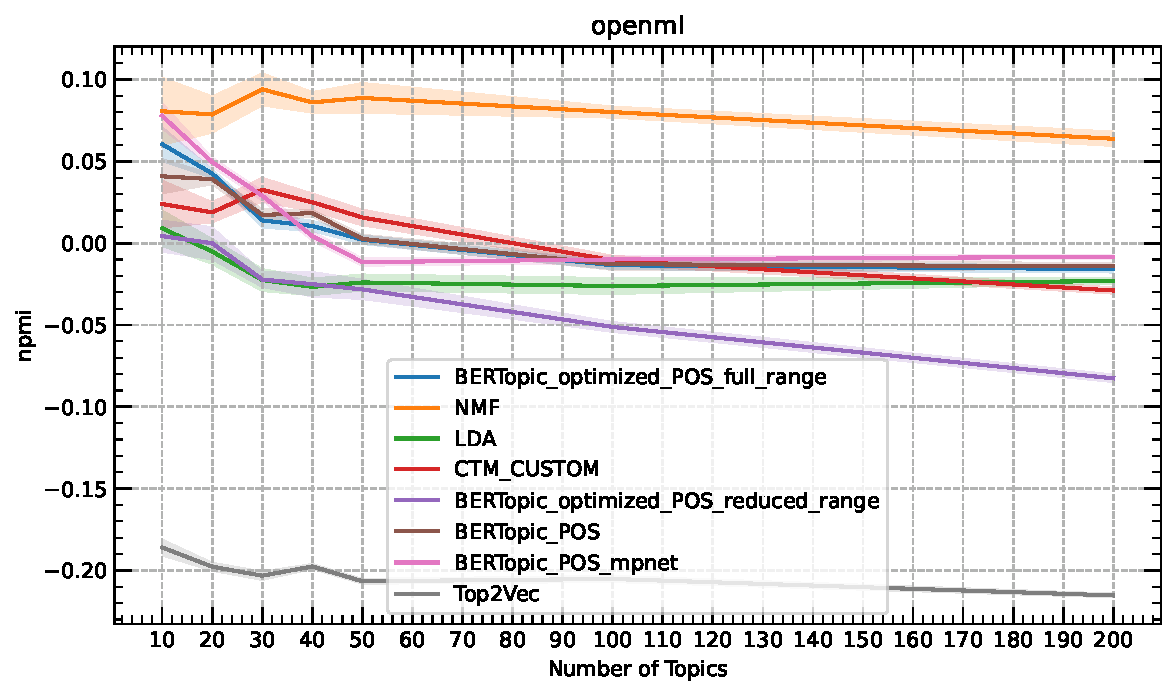
\includegraphics[width=0.85\textwidth]{figures/openml_npmi.pdf}
    \caption{Line chart of the NPMI scores for the hyperparameter-optimized BERTopic model and the baseline models}
    \label{fig:openml_npmi}
\end{figure}

We observe that the NMF model outperforms all models across all topic numbers. However, when we look at \cref{fig:openml_diversity}, we see that the NMF model has very low diversity scores. This suggests that the NMF model may be picking the same terms in each topic, leading to high coherence but low diversity. For NPMI, we then see that the BERTopic models perform the second best, with very small differences between them. We see that \textbf{BERTopic\_optimized\_POS\_reduced\_range} performs slightly worse, but this is likely due to the smaller topic sizes we explored. We see that LDA, CTM, and Top2Vec perform worse than the BERTopic models.

As for diversity, we see that the \textbf{BERTopic\_optimized\_POS\_full\_range} has the highest diversity scores, followed by the other BERTopic models. This suggests that the BERTopic models are able to capture a wider range of terms in their topics compared to the other models. Surprisingly, the Top2Vec model has the lowest NPMI and diversity scores.

\begin{figure}[h]
    \centering
    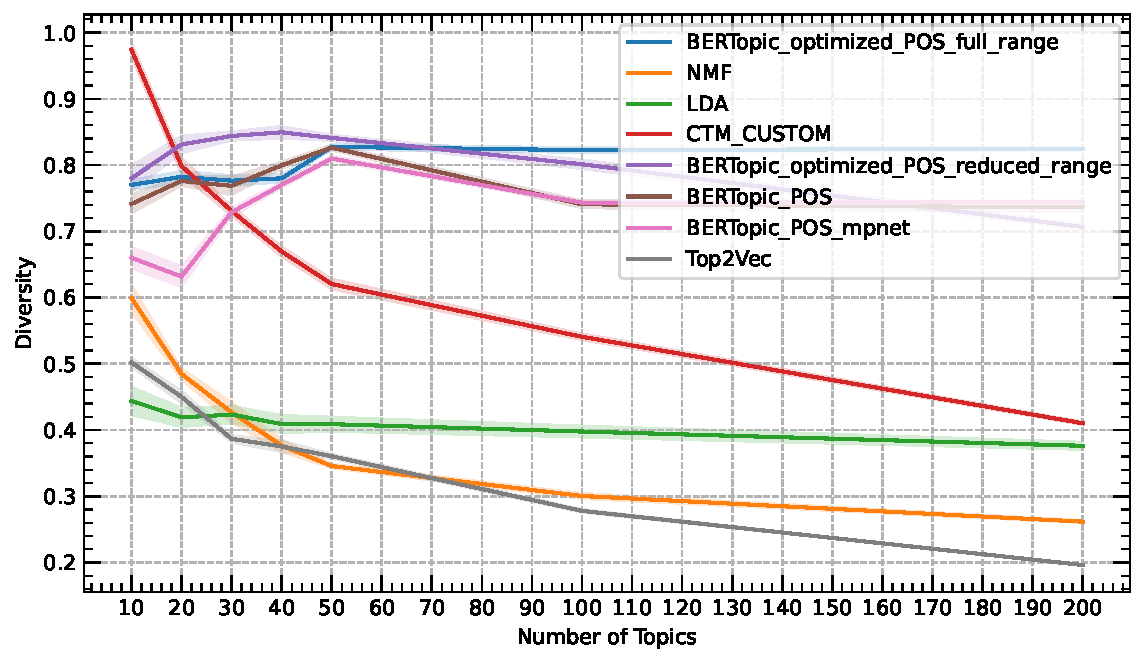
\includegraphics[width=0.85\textwidth]{figures/openml_diversity.pdf}
    \caption{Line chart of the diversity scores for the hyperparameter-optimized BERTopic model and the baseline models}
    \label{fig:openml_diversity}
\end{figure}

In \cref{tab:openml_results}, we present the NPMI and diversity scores for the models. We highlight the best scores in dark green and the subsequent best scores in lighter green. We see that the BERTopic models perform well in terms of diversity, with the \textbf{BERTopic\_optimized\_POS\_reduced\_range} model having the highest diversity score. If we only look at the BERTopic models, we can note a strong negative Pearson correlation between NPMI and diversity scores of -0.67. This suggests that the higher coherence may be driven by the inclusion of more common terms in the topics, while the diversity score is driven by the inclusion of more unique terms. In any case, the BERTopic models outperform the baseline models in terms of combined NPMI and diversity scores.

\begin{table}[h]
    \centering
    \definecolor{color64db00}{HTML}{64db00}
    \definecolor{color76FF03}{HTML}{76FF03}
    \definecolor{colore1ffc7}{HTML}{e1ffc7}
    \begin{tabular}{>{\centering\arraybackslash}m{25em}>{\centering\arraybackslash}m{7em}>{\centering\arraybackslash}m{7em}}
        \toprule
        \textbf{Model}                           & \textbf{npmi}                 & \textbf{diversity}            \\
        \midrule
        Top2Vec                                  & -0.202                        & 0.364                         \\
        BERTopic\_optimized\_POS\_reduced\_range & -0.029                        & \cellcolor{color64db00} 0.808 \\
        LDA                                      & -0.017                        & 0.411                         \\
        CTM\_CUSTOM                              & 0.011                         & 0.678                         \\
        BERTopic\_POS                            & 0.013                         & \cellcolor{colore1ffc7} 0.770 \\
        BERTopic\_optimized\_POS\_full\_range    & \cellcolor{colore1ffc7} 0.014 & \cellcolor{color76FF03} 0.798 \\
        BERTopic\_POS\_mpnet                     & \cellcolor{color76FF03} 0.019 & 0.727                         \\
        NMF                                      & \cellcolor{color64db00} 0.082 & 0.399                         \\
        \bottomrule
    \end{tabular}
    \caption{NPMI and diversity scores for the hyperparameter-optimized BERTopic model and the baseline models}
    \label{tab:openml_results}
\end{table}

\subsubsection{Statistical significance}
As mentioned earlier, we had 10 runs for each model and topic number combination. We will now assess whether there are statistically significant differences between the performance of the models. We check whether the assumptions for ANOVA are met, and if not, we use Welch's ANOVA or Kruskal-Wallis (non-parametric) tests.

The first assumption for ANOVA is that the residuals are normally distributed. We apply the Shapiro-Wilk test to check whether the residuals for the NPMI values (the differences between the observed and predicted NPMI values) are normally distributed. The Shapiro-Wilk test returned a statistic of 0.905 and a p-value of 3.30e-18, indicating a significant deviation from normality. Although the statistic is relatively close to 1, suggesting that the residuals are not drastically non-normal, the extremely small p-value suggests that the deviation is statistically significant. As for the diversity values, the Shapiro-Wilk test returned a statistic of 0.968 and a p-value of 8.70e-10, also indicating a significant deviation from normality, but with a statistic even closer to 1.

Given this result, we further inspect the residuals using visual diagnostics with QQ plots and histograms to assess the nature and extent of the deviation from normality. If the deviation is minor, ANOVA may still be appropriate. \cref{fig:qqplot_npmi} and \cref{fig:histogram_npmi} show the QQ plot and histogram of the residuals for the NPMI values, respectively. We observe that the residuals are approximately normally distributed, with some deviations at the tails. \cref{fig:qqplot_diversity} and \cref{fig:histogram_diversity} show the QQ plot and histogram of the residuals for the diversity values, respectively. We observe a similar pattern for the diversity residuals, with some deviations at the tails. Given that ANOVA is relatively robust to deviations at the tails, since extreme values do not have a large impact on the F-statistic, we consider this assumption to be met.

\begin{figure}[h]
    \centering
    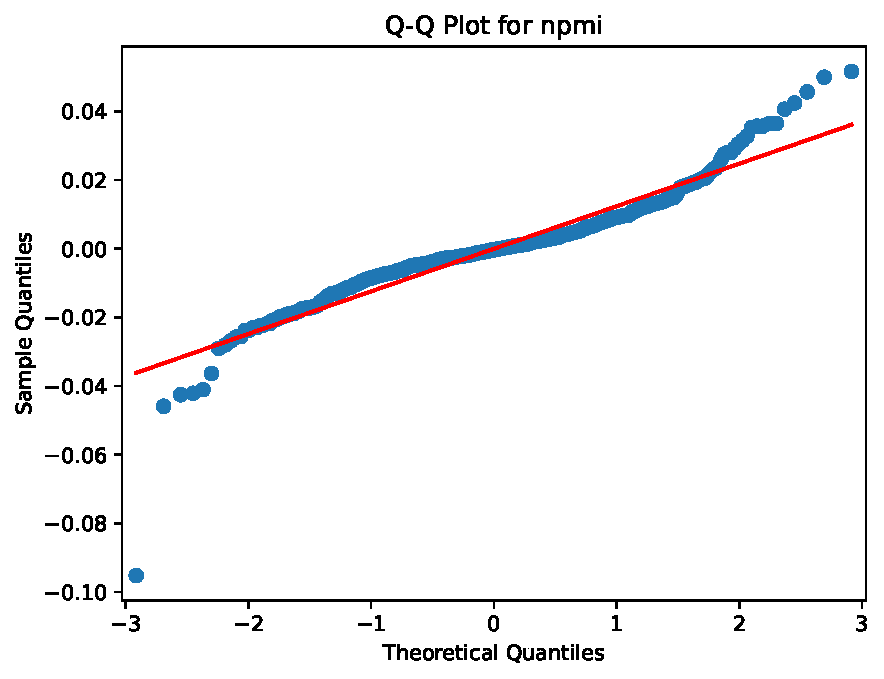
\includegraphics[width=0.85\textwidth]{figures/qqplot_npmi.pdf}
    \caption{QQ plot of the residuals for the NPMI values}
    \label{fig:qqplot_npmi}
\end{figure}

\begin{figure}[h]
    \centering
    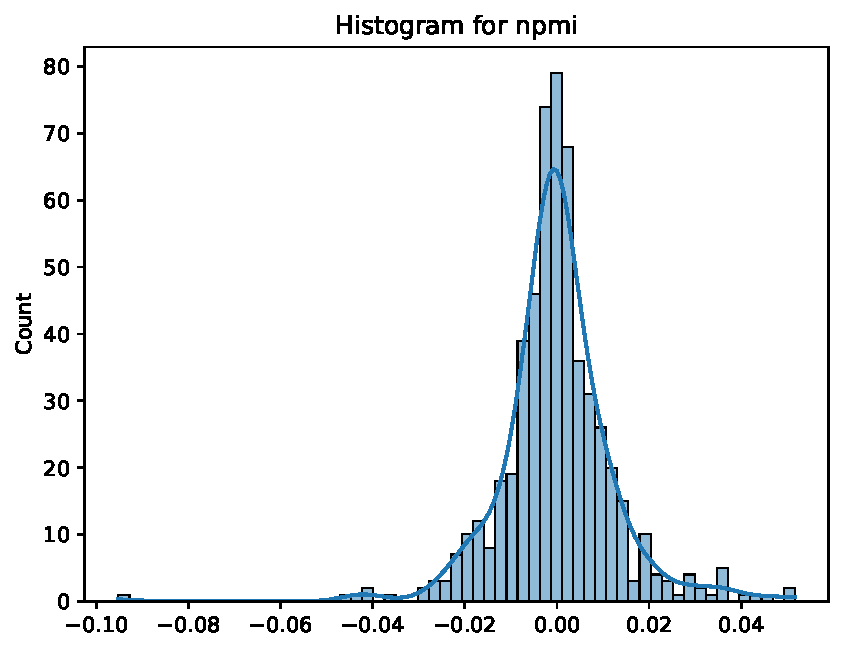
\includegraphics[width=0.85\textwidth]{figures/histogram_npmi.pdf}
    \caption{Histogram of the residuals for the NPMI values}
    \label{fig:histogram_npmi}
\end{figure}

\begin{figure}[h]
    \centering
    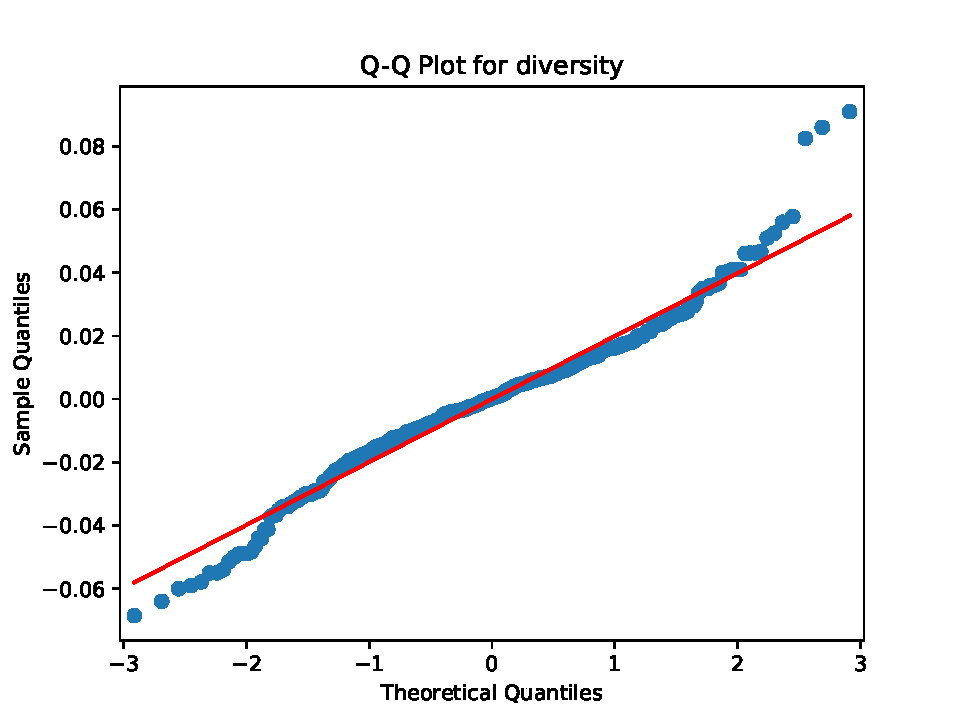
\includegraphics[width=0.85\textwidth]{figures/qqplot_diversity.pdf}
    \caption{QQ plot of the residuals for the diversity values}
    \label{fig:qqplot_diversity}
\end{figure}

\begin{figure}[h]
    \centering
    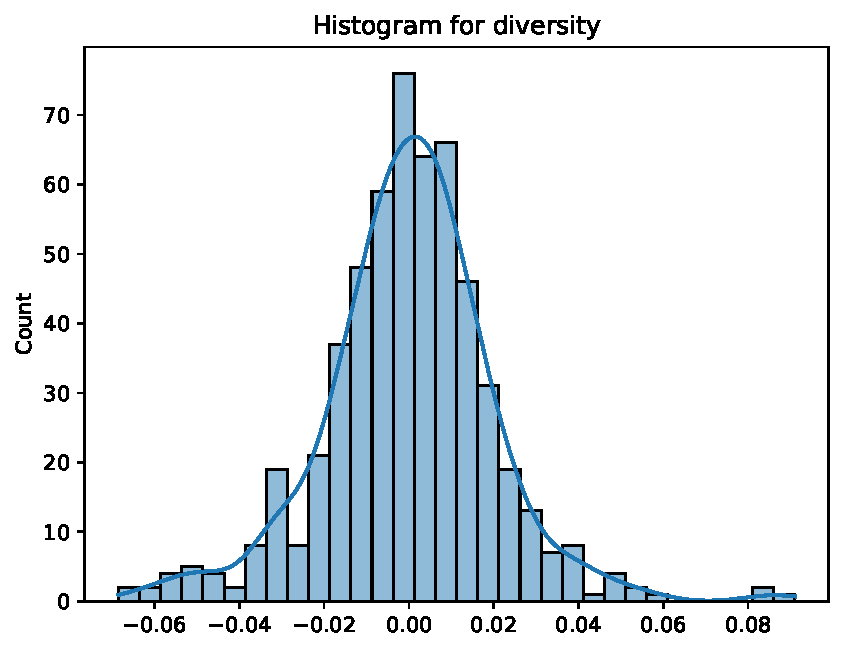
\includegraphics[width=0.85\textwidth]{figures/histogram_diversity.pdf}
    \caption{Histogram of the residuals for the diversity values}
    \label{fig:histogram_diversity}
\end{figure}

The second assumption for ANOVA is that the residuals have equal variance. We apply the Levene test and the Bartlett test to check whether the residuals have equal variance, for each model and topic number combination. \cref{tab:levene_bartlett} shows the results of the Levene and Bartlett tests for the NPMI and diversity values. We observe that the p-values are mostly below 0.05, indicating that the residuals do not have equal variance. This violates the assumption of homoscedasticity (equal variance) for ANOVA. Therefore, we will use Welch's ANOVA, since the first assumption is met, and the residuals are approximately normally distributed, but the assumption of equal variance is violated.

\begin{table}[htbp]
    \centering
    \caption{Levene's and Bartlett's Tests for NPMI and Diversity}
    \begin{tabular}{@{}lcc|cc@{}}
        \toprule
                            & \multicolumn{2}{c}{\textbf{NPMI}} & \multicolumn{2}{c}{\textbf{Diversity}}                                         \\ \cmidrule(lr){2-3} \cmidrule(lr){4-5}
        \textbf{nr\_topics} & \textbf{Statistic}                & \textbf{p-value}                       & \textbf{Statistic} & \textbf{p-value} \\ \midrule
        \multicolumn{5}{c}{\textbf{Levene's Test}}                                                                                               \\ \midrule
        10                  & 1.4665                            & 0.1930                                 & 1.6530             & 0.1346           \\
        20                  & 4.0018                            & 0.0009                                 & 1.2666             & 0.2791           \\
        30                  & 2.9904                            & 0.0082                                 & 2.0219             & 0.0638           \\
        40                  & 2.6662                            & 0.0164                                 & 1.1821             & 0.3239           \\
        50                  & 2.9896                            & 0.0082                                 & 2.5184             & 0.0225           \\
        100                 & 1.0988                            & 0.3733                                 & 1.4504             & 0.1990           \\
        200                 & 2.4367                            & 0.0268                                 & 2.6070             & 0.0186           \\ \midrule
        \multicolumn{5}{c}{\textbf{Bartlett's Test}}                                                                                             \\ \midrule
        10                  & 19.3408                           & 0.0072                                 & 17.4000            & 0.0150           \\
        20                  & 39.6442                           & 1.4724e-06                             & 7.5180             & 0.3770           \\
        30                  & 24.0258                           & 0.0011                                 & 14.8213            & 0.0384           \\
        40                  & 27.6841                           & 0.0003                                 & 11.7576            & 0.1088           \\
        50                  & 34.6455                           & 1.3038e-05                             & 19.0298            & 0.0081           \\
        100                 & 9.8099                            & 0.1996                                 & 15.5252            & 0.0298           \\
        200                 & 20.3993                           & 0.0048                                 & 31.0744            & 6.0240e-05       \\ \bottomrule
    \end{tabular}
    \label{tab:levene_bartlett}
\end{table}

Applying Welch's ANOVA to the NPMI and diversity values, we find that there are statistically significant differences between the models for both metrics (\cref{tab:welch_anova}). For NPMI, 90.75\% of the variance is explained by the model, and for diversity, 81.50\% of the variance is explained by the model. These are both large effect sizes, suggesting that the models have a substantial impact on both metrics.

We then perform post-hoc tests to determine which models are significantly different from one another. We use the Games-Howell post-hoc test, which is appropriate when the assumption of equal variance is violated. The results of the Games-Howell post-hoc test for the NPMI values are shown in \cref{tab:games_howell_npmi}. We observe that the BERTopic models are significantly different from the other models, but generally not much from each other. Similarly, the results of the Games-Howell post-hoc test for the diversity values are shown in \cref{tab:games_howell_diversity}. We observe that the BERTopic models are significantly different from the other models, but not from each other.

\begin{table}[ht]
    \centering
    \caption{Welch's ANOVA Results for NPMI and Diversity}
    \label{tab:welch_anova}
    \begin{tabular}{lcccccc}
        \toprule
        \textbf{Metric}    & \textbf{Source} & \textbf{df1} & \textbf{df2} & \textbf{F-value} & \textbf{p-value}            & \textbf{np2} \\
        \midrule
        \textbf{NPMI}      & Model           & 7            & 231.601      & 2549.36          & $3.165650 \times 10^{-215}$ & 0.90749      \\
        \textbf{Diversity} & Model           & 7            & 232.705      & 1091.24          & $4.954462 \times 10^{-174}$ & 0.815016     \\
        \bottomrule
    \end{tabular}
\end{table}

\begin{table}[ht]
    \centering
    \caption{Games-Howell Post-hoc Test Results for NPMI}
    \label{tab:games_howell_npmi}
    \begin{tabular}{lccc}
        \toprule
        \textbf{Comparison (A vs. B)}              & \textbf{Diff} & \textbf{p-value} & \textbf{Hedges' g} \\
        \midrule
        \textbf{B\_POS vs. B\_POS\_mpnet}          & -0.0057       & 0.9385           & -0.197             \\
        \textbf{B\_POS vs. B\_OPT\_FULL}           & -0.0013       & 0.999988         & -0.050             \\
        \textbf{B\_POS vs. B\_OPT\_REDUCED}        & 0.0423        & 1.498801e-14     & 1.546              \\
        \textbf{B\_POS vs. CTM}                    & 0.0021        & 0.999622         & 0.085              \\
        \textbf{B\_POS vs. LDA}                    & 0.0300        & 7.661649e-13     & 1.439              \\
        \textbf{B\_POS vs. NMF}                    & -0.0687       & 4.252154e-14     & -2.993             \\
        \textbf{B\_POS vs. Top2Vec}                & 0.2147        & 0.000000         & 12.024             \\
        \textbf{B\_POS\_mpnet vs. B\_OPT\_FULL}    & 0.0044        & 0.990508         & 0.141              \\
        \textbf{B\_POS\_mpnet vs. B\_OPT\_REDUCED} & 0.0480        & 1.374456e-13     & 1.488              \\
        \textbf{B\_POS\_mpnet vs. CTM}             & 0.0077        & 0.779209         & 0.260              \\
        \textbf{B\_POS\_mpnet vs. LDA}             & 0.0356        & 8.421752e-11     & 1.324              \\
        \textbf{B\_POS\_mpnet vs. NMF}             & -0.0630       & 3.841372e-14     & -2.205             \\
        \textbf{B\_POS\_mpnet vs. Top2Vec}         & 0.2203        & 0.000000         & 8.929              \\
        \textbf{B\_OPT\_FULL vs. B\_OPT\_REDUCED}  & 0.0436        & 1.706413e-13     & 1.471              \\
        \textbf{B\_OPT\_FULL vs. CTM}              & 0.0034        & 0.995362         & 0.125              \\
        \textbf{B\_OPT\_FULL vs. LDA}              & 0.0313        & 6.274092e-11     & 1.317              \\
        \textbf{B\_OPT\_FULL vs. NMF}              & -0.0674       & 0.000000         & -2.631             \\
        \textbf{B\_OPT\_FULL vs. Top2Vec}          & 0.2160        & 1.643130e-14     & 10.202             \\
        \textbf{B\_OPT\_REDUCED vs. CTM}           & -0.0403       & 1.185607e-12     & -1.422             \\
        \textbf{B\_OPT\_REDUCED vs. LDA}           & -0.0124       & 0.085287         & -0.485             \\
        \textbf{B\_OPT\_REDUCED vs. NMF}           & -0.1110       & 1.110223e-16     & -4.074             \\
        \textbf{B\_OPT\_REDUCED vs. Top2Vec}       & 0.1724        & 6.661338e-16     & 7.455              \\
        \textbf{CTM vs. LDA}                       & 0.0279        & 2.411494e-10     & 1.266              \\
        \textbf{CTM vs. NMF}                       & -0.0707       & 0.000000         & -2.940             \\
        \textbf{CTM vs. Top2Vec}                   & 0.2126        & 9.992007e-15     & 11.039             \\
        \textbf{LDA vs. NMF}                       & -0.0987       & 0.000000         & -4.776             \\
        \textbf{LDA vs. Top2Vec}                   & 0.1847        & 0.000000         & 12.492             \\
        \textbf{NMF vs. Top2Vec}                   & 0.2834        & 1.543210e-14     & 16.054             \\
        \bottomrule
    \end{tabular}
\end{table}

\begin{table}[ht]
    \centering
    \caption{Games-Howell Post-hoc Test Results for Diversity}
    \label{tab:games_howell_diversity}
    \begin{tabular}{lccc}
        \toprule
        \textbf{Comparison (A vs. B)}              & \textbf{Diff} & \textbf{p-value} & \textbf{Hedges' g} \\
        \midrule
        \textbf{B\_POS vs. B\_POS\_mpnet}          & 0.0431        & 0.000041         & 0.853              \\
        \textbf{B\_POS vs. B\_OPT\_FULL}           & -0.0278       & 0.000044         & -0.845             \\
        \textbf{B\_POS vs. B\_OPT\_REDUCED}        & -0.0378       & 0.000072         & -0.827             \\
        \textbf{B\_POS vs. CTM}                    & 0.0921        & 0.000849         & 0.741              \\
        \textbf{B\_POS vs. LDA}                    & 0.3587        & 4.329870e-15     & 10.075             \\
        \textbf{B\_POS vs. NMF}                    & 0.3706        & 3.330669e-15     & 4.486              \\
        \textbf{B\_POS vs. Top2Vec}                & 0.4058        & 4.107825e-15     & 5.537              \\
        \textbf{B\_POS\_mpnet vs. B\_OPT\_FULL}    & -0.0709       & 1.008860e-12     & -1.494             \\
        \textbf{B\_POS\_mpnet vs. B\_OPT\_REDUCED} & -0.0809       & 1.283196e-12     & -1.417             \\
        \textbf{B\_POS\_mpnet vs. CTM}             & 0.0490        & 0.326768         & 0.380              \\
        \textbf{B\_POS\_mpnet vs. LDA}             & 0.3156        & 1.221245e-15     & 6.387              \\
        \textbf{B\_POS\_mpnet vs. NMF}             & 0.3275        & 2.609024e-14     & 3.662              \\
        \textbf{B\_POS\_mpnet vs. Top2Vec}         & 0.3627        & 1.887379e-15     & 4.483              \\
        \textbf{B\_OPT\_FULL vs. B\_OPT\_REDUCED}  & -0.0100       & 0.852516         & -0.236             \\
        \textbf{B\_OPT\_FULL vs. CTM}              & 0.1199        & 4.375404e-06     & 0.975              \\
        \textbf{B\_OPT\_FULL vs. LDA}              & 0.3865        & 0.000000         & 12.439             \\
        \textbf{B\_OPT\_FULL vs. NMF}              & 0.3984        & 0.000000         & 4.933              \\
        \textbf{B\_OPT\_FULL vs. Top2Vec}          & 0.4336        & 0.000000         & 6.090              \\
        \textbf{B\_OPT\_REDUCED vs. CTM}           & 0.1299        & 9.880746e-07     & 1.023              \\
        \textbf{B\_OPT\_REDUCED vs. LDA}           & 0.3965        & 0.000000         & 8.929              \\
        \textbf{B\_OPT\_REDUCED vs. NMF}           & 0.4084        & 0.000000         & 4.707              \\
        \textbf{B\_OPT\_REDUCED vs. Top2Vec}       & 0.4436        & 2.919887e-14     & 5.691              \\
        \textbf{CTM vs. LDA}                       & 0.2666        & 0.000000         & 2.154              \\
        \textbf{CTM vs. NMF}                       & 0.2785        & 5.573320e-14     & 1.928              \\
        \textbf{CTM vs. Top2Vec}                   & 0.3137        & 0.000000         & 2.251              \\
        \textbf{LDA vs. NMF}                       & 0.0120        & 9.880892e-01     & 0.146              \\
        \textbf{LDA vs. Top2Vec}                   & 0.0471        & 5.115797e-03     & 0.649              \\
        \textbf{NMF vs. Top2Vec}                   & 0.0351        & 4.794142e-01     & 0.338              \\
        \bottomrule
    \end{tabular}
\end{table}

\section{Tag Generation}
In \cref{sec:tag_generation} and \cref{fig:tag_generation_pipeline}, we presented the tag generation pipeline on a high level. \cref{fig:tag_generation_pipeline_specifics}, which is similar to \cref{fig:tag_generation_pipeline} shows the specifics of the tag generation pipeline. In particular, we show which specific submodels we used for the different steps in the pipeline:
\begin{enumerate}
    \item \textbf{Original Descriptions}: Same as in the high-level pipeline, we start with the original OpenML dataset descriptions.
    \item \textbf{Augmented Descriptions}: In \cref{sec:data_exploration}, we discussed how we augment the descriptions with additional information.
    \item \textbf{Prompt Descriptions Human-Readable}: For this step, we used the \texttt{Llama-3-70b} model, as it was a model offering a good balance between performance and computational resources at the time of the experiment. We engineered a prompt to extract keyword tags from each individual description. We do not include the prompt here for brevity, but it is available in the \href{https://github.com/ivangermanov/openml-tags}{GitHub repository} \cite{germanov_topic_modeling_of_2024}.
    \item \textbf{Create Embeddings}: We use the \texttt{Salesforce/SFR-Embedding-2\_R} model, which was the best performing model on the MTEB benchmark \cite{muennighoff_mteb_2023}.
    \item \textbf{Base BERTopic Model}: For dimensionality reduction, clustering, bag-of-words construction and c-TF-IDF calculation, we use the hyperparameter-optimized BERTopic model.
    \item \textbf{Fine-tune to Extract Tags}: For the fine-tuning step, we use the \texttt{Llama-3-70b} model. We prompt the model to generate tags for each cluster. The prompt can again be found in the repository.
    \item \textbf{Zeroshot Classifier}: We use the \texttt{MoritzLaurer/deberta-v3-large-zeroshot-v2.0} model \cite{noauthor_moritzlaurerdeberta-v3-large-zeroshot-v20_2024}, which at the time of the experiment was the best performing model for the zeroshot text classification task.
\end{enumerate}

\begin{figure}[h]
    \centering
    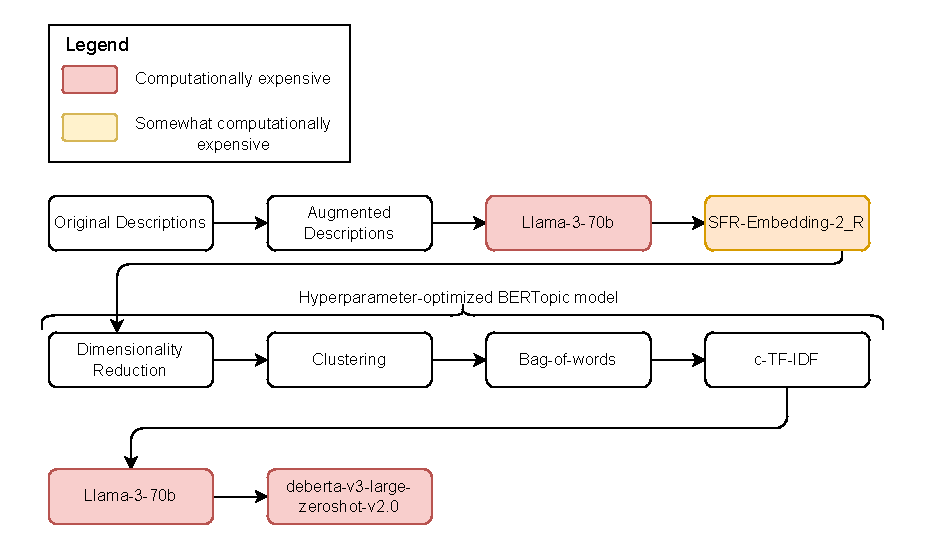
\includegraphics[width=\textwidth]{figures/tag_generation_pipeline_specifics.pdf}
    \caption{Tag generation pipeline specifics}
    \label{fig:tag_generation_pipeline_specifics}
\end{figure}

\subsection{Results}
We now show the results of the output of the tag generation pipeline. \cref{fig:top_50_frequency} shows the top 50 regular tags by frequency, while \cref{fig:top_50_overarching_frequency} shows the top 50 overarching tags by frequency. We see that the tags are quite diverse, covering a wide range of topics. The regular tags are more specific, while the overarching tags are more general.

\begin{figure}[h]
    \centering
    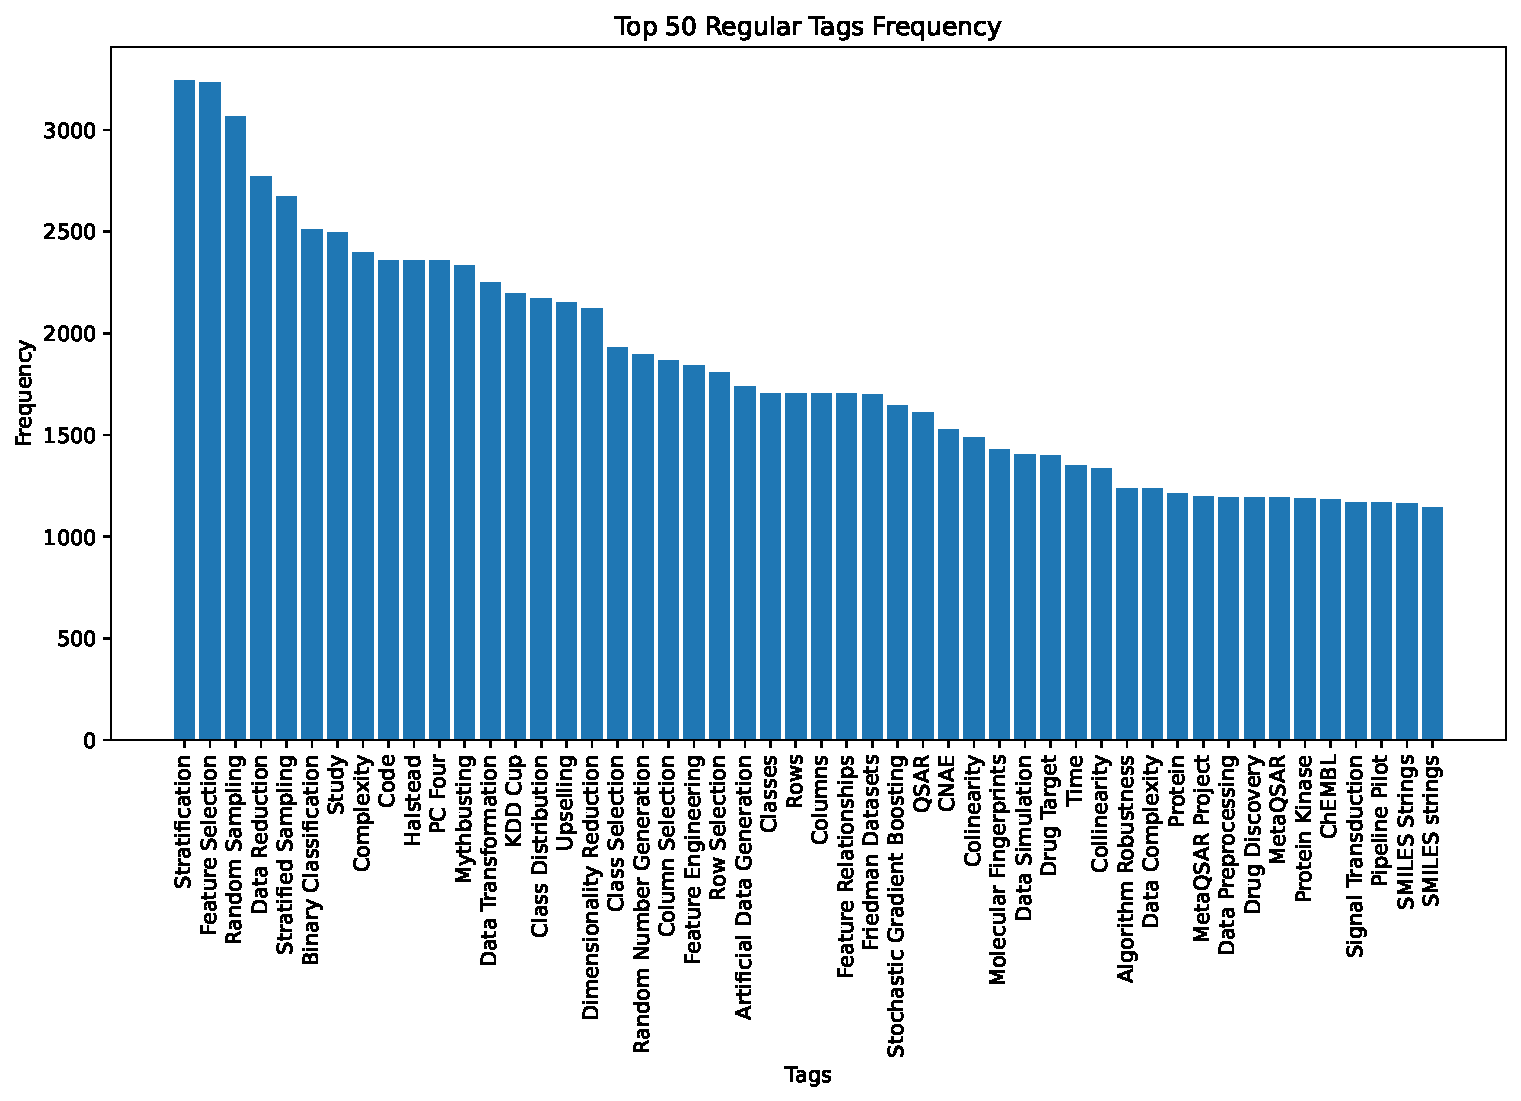
\includegraphics[width=\textwidth]{figures/top_50_frequency.pdf}
    \caption{Top 50 tags by frequency}
    \label{fig:top_50_frequency}
\end{figure}

\begin{figure}[h]
    \centering
    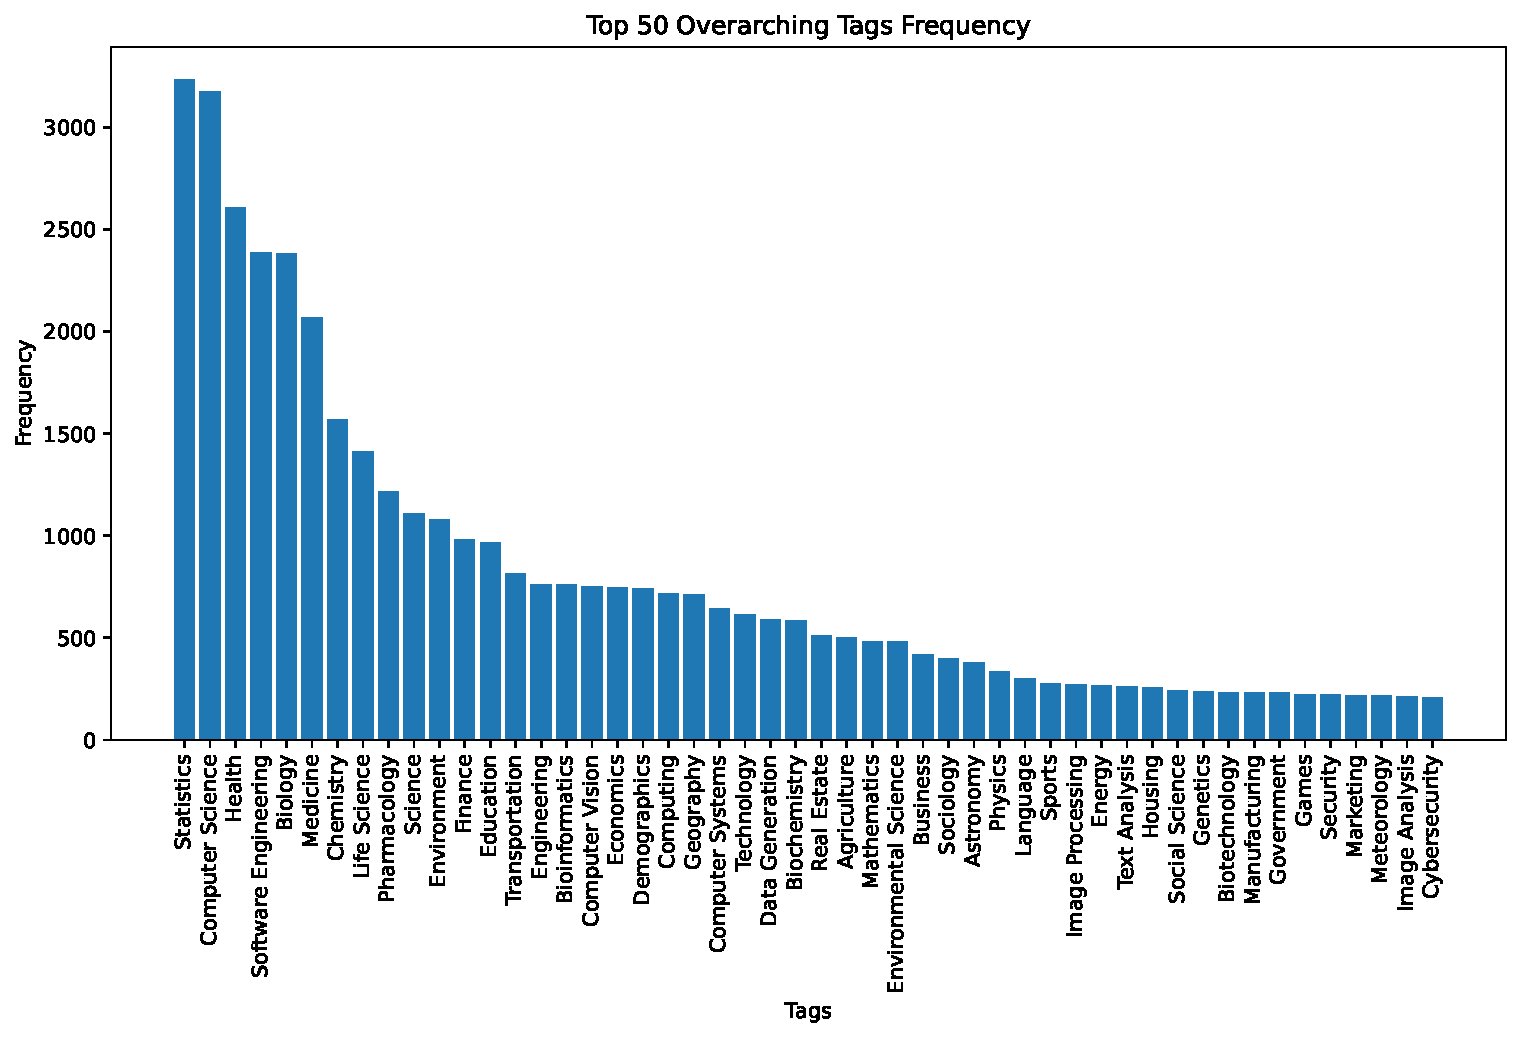
\includegraphics[width=\textwidth]{figures/top_50_overarching_frequency.pdf}
    \caption{Top 50 overarching tags by frequency}
    \label{fig:top_50_overarching_frequency}
\end{figure}

Investigating the tag counts in more detail, we see that the distribution of the tags is highly skewed. \cref{fig:box_plot_tag_counts} shows a box plot of the tag counts, while \cref{fig:box_plot_overarching_tag_counts} shows a box plot of the overarching tag counts. We see that the majority of tags have a low count, with a few tags having a very high count. This is expected, as natural language has been found to follow Zipf's law (Zipfian distribution), where a few terms are very common, while the majority of terms are rare \cite{zipf_psycho-biology_1935, piantadosi_zipfs_2014}.

\begin{figure}[h]
    \centering
    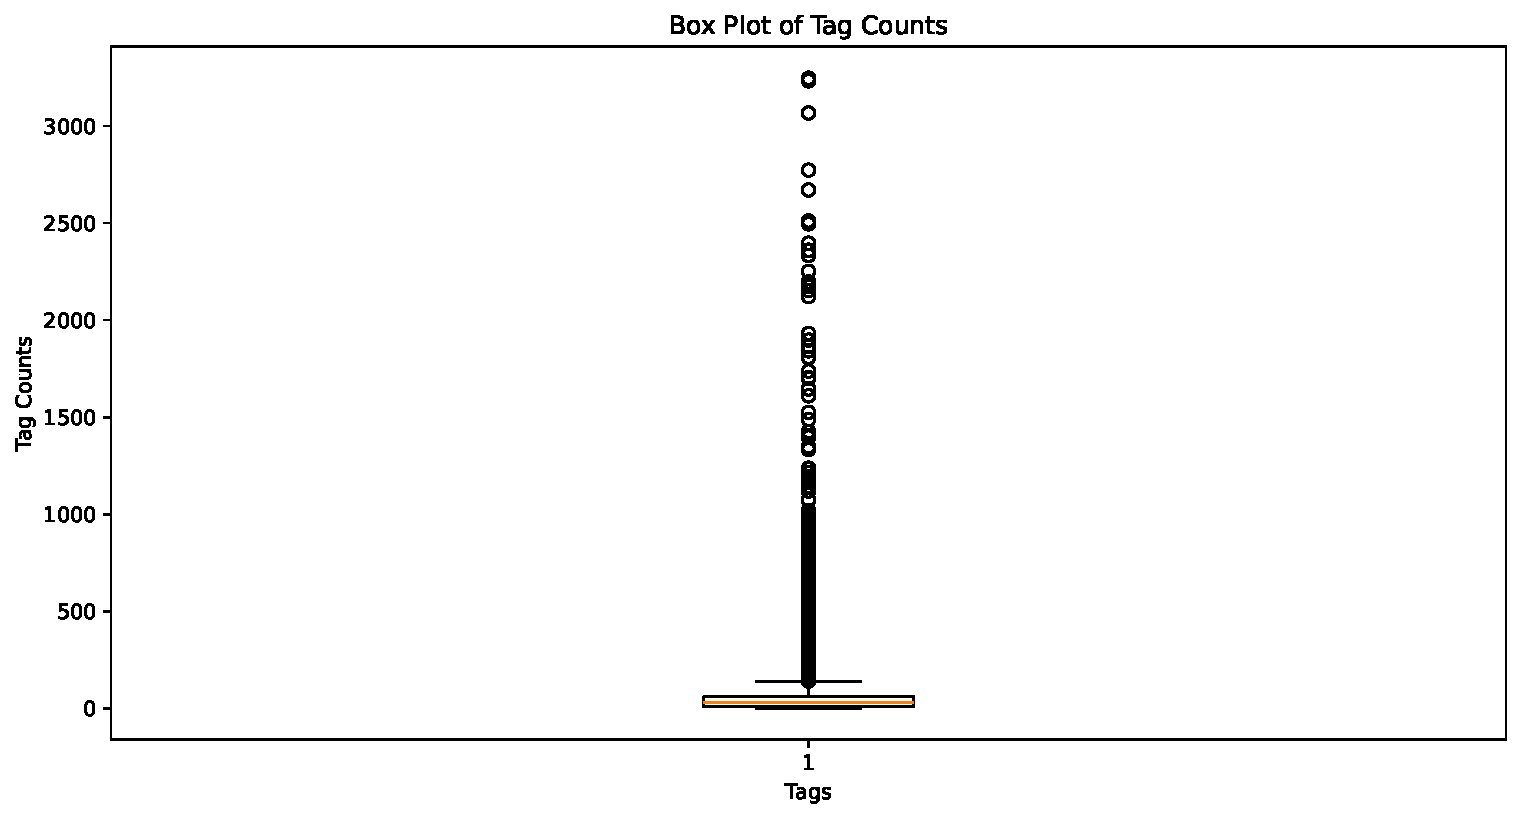
\includegraphics[width=\textwidth]{figures/box_plot_tag_counts.pdf}
    \caption{Box plot of tag counts}
    \label{fig:box_plot_tag_counts}
\end{figure}

\begin{figure}[h]
    \centering
    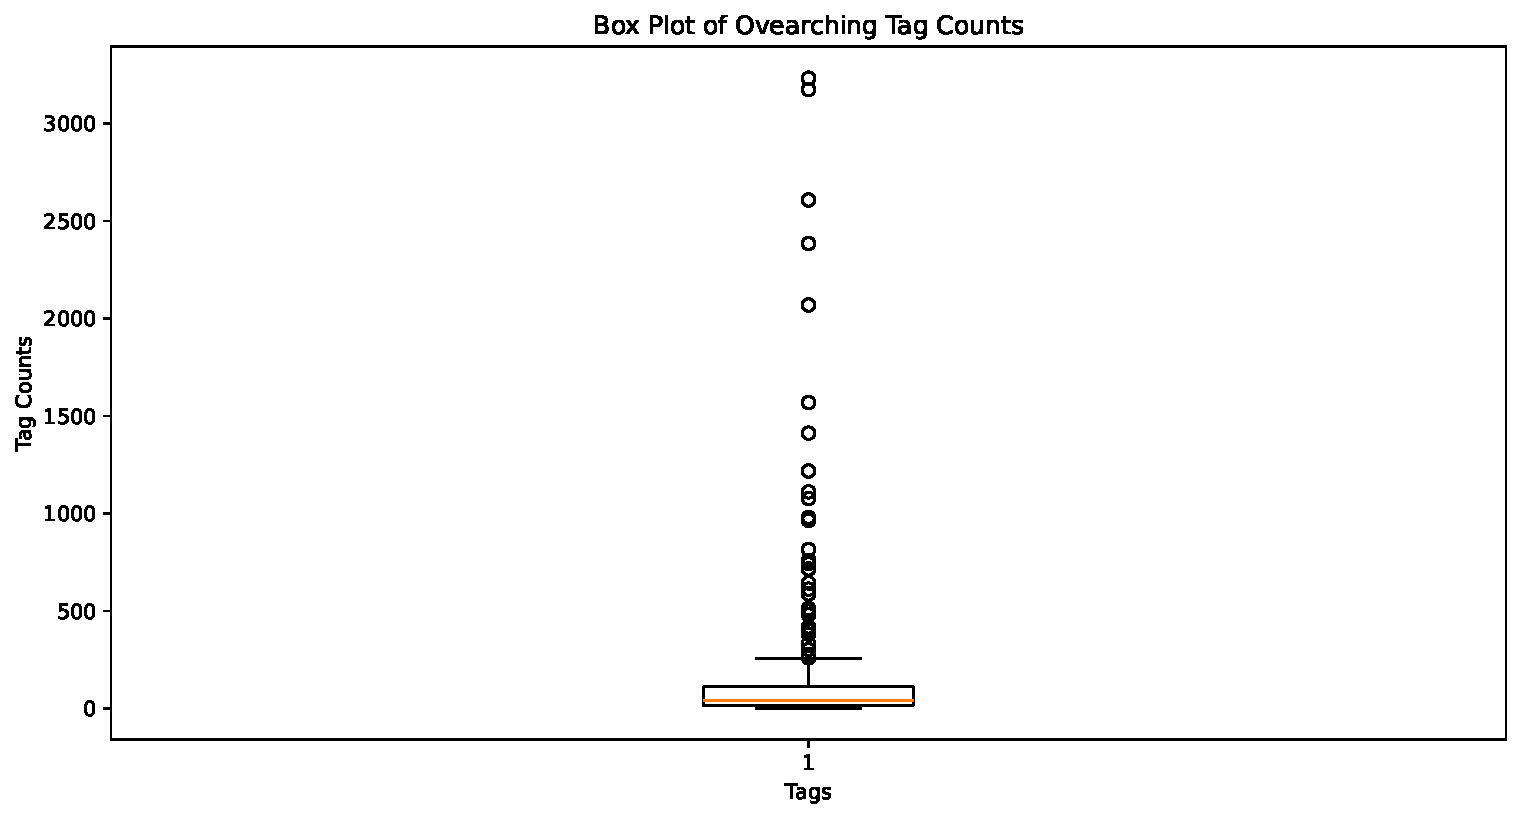
\includegraphics[width=\textwidth]{figures/box_plot_overarching_tag_counts.pdf}
    \caption{Box plot of overarching tag counts}
    \label{fig:box_plot_overarching_tag_counts}
\end{figure}

We observe the same pattern when looking at histograms of the tag counts. \cref{fig:histogram_tag_counts} shows the histogram of tag counts, while \cref{fig:histogram_tag_counts_log} shows the histogram of tag counts on a log scale. We see that the distribution is highly skewed, with a few tags having a very high count. In \cref{fig:histogram_overarching_tag_counts} and \cref{fig:histogram_overarching_tag_counts_log}, we see the same pattern for the overarching tags. It is important to note that the number of regular tags is approx. 6300 and the number of overarching tags is approx. 300. This is also expected, as the overarching tags are more general and should cover a wider range of topics.

\begin{figure}[h]
    \centering
    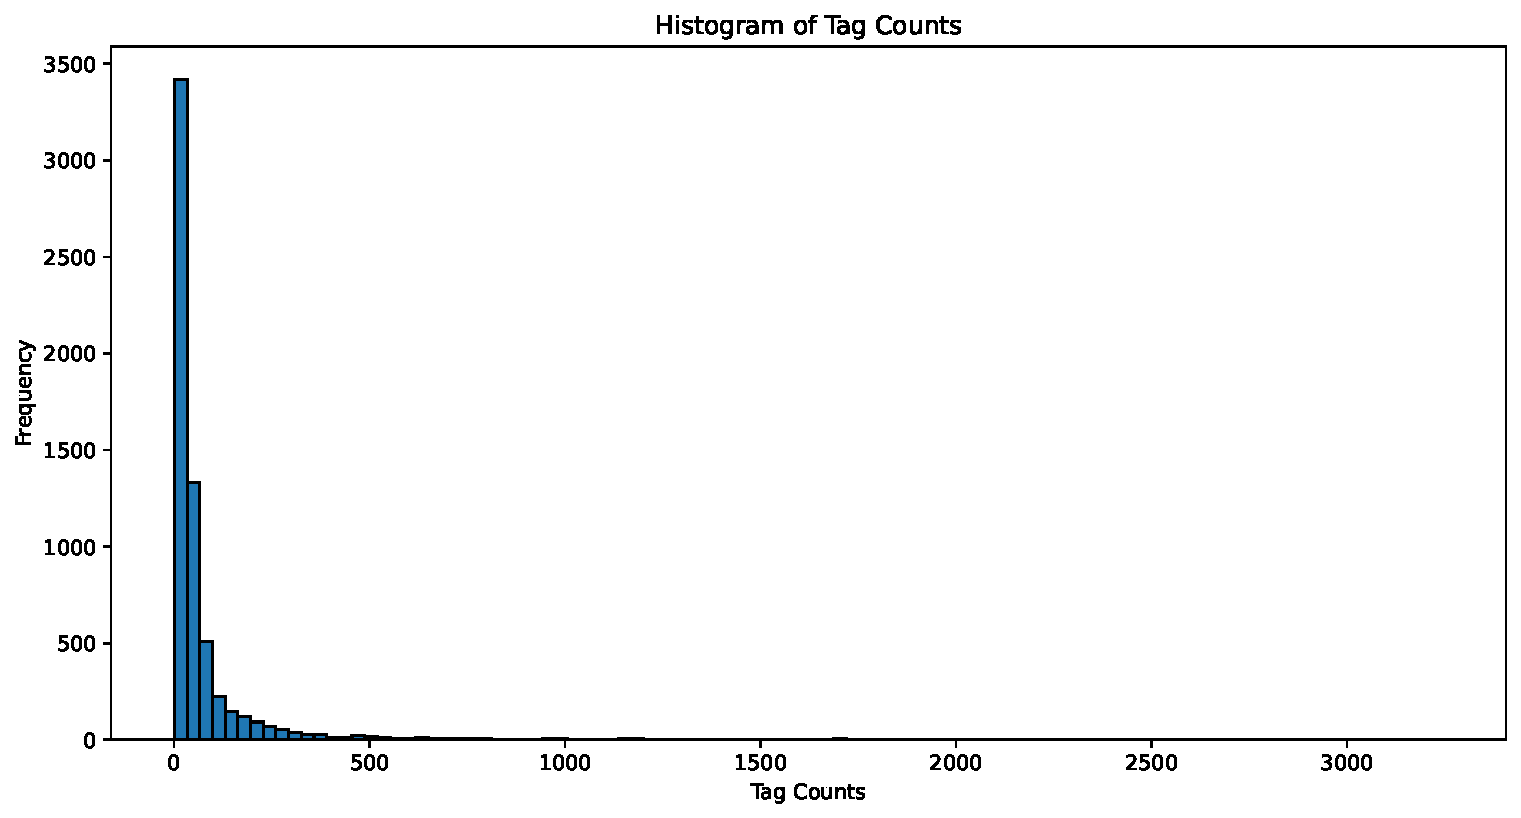
\includegraphics[width=\textwidth]{figures/histogram_tag_counts.pdf}
    \caption{Histogram of tag counts}
    \label{fig:histogram_tag_counts}
\end{figure}

\begin{figure}[h]
    \centering
    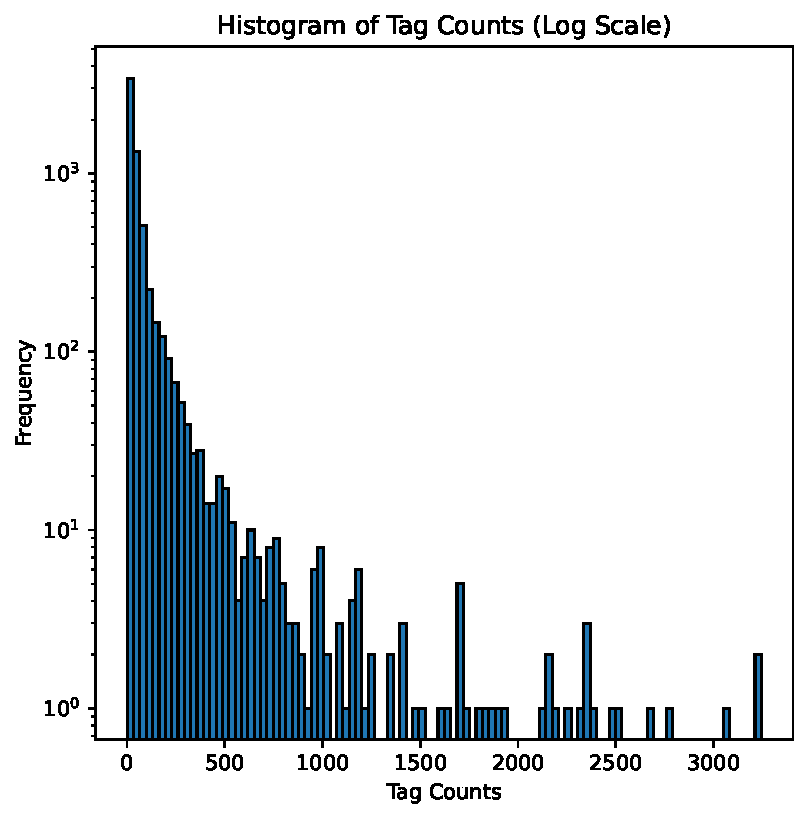
\includegraphics[width=\textwidth]{figures/histogram_tag_counts_log.pdf}
    \caption{Histogram of tag counts (log scale)}
    \label{fig:histogram_tag_counts_log}
\end{figure}

\begin{figure}[h]
    \centering
    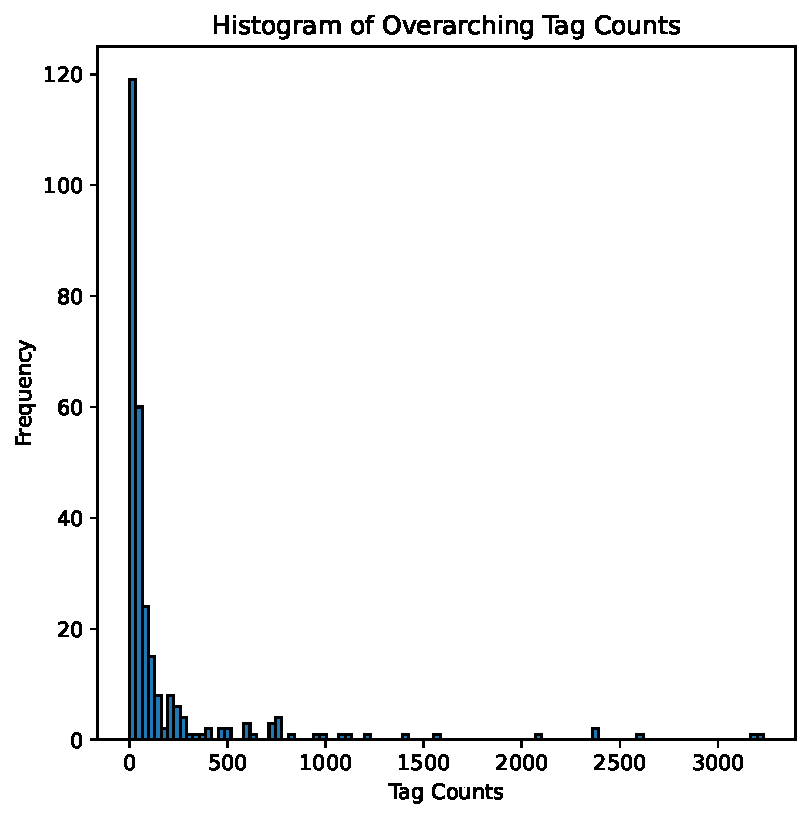
\includegraphics[width=\textwidth]{figures/histogram_overarching_tag_counts.pdf}
    \caption{Histogram of overarching tag counts}
    \label{fig:histogram_overarching_tag_counts}
\end{figure}

\begin{figure}[h]
    \centering
    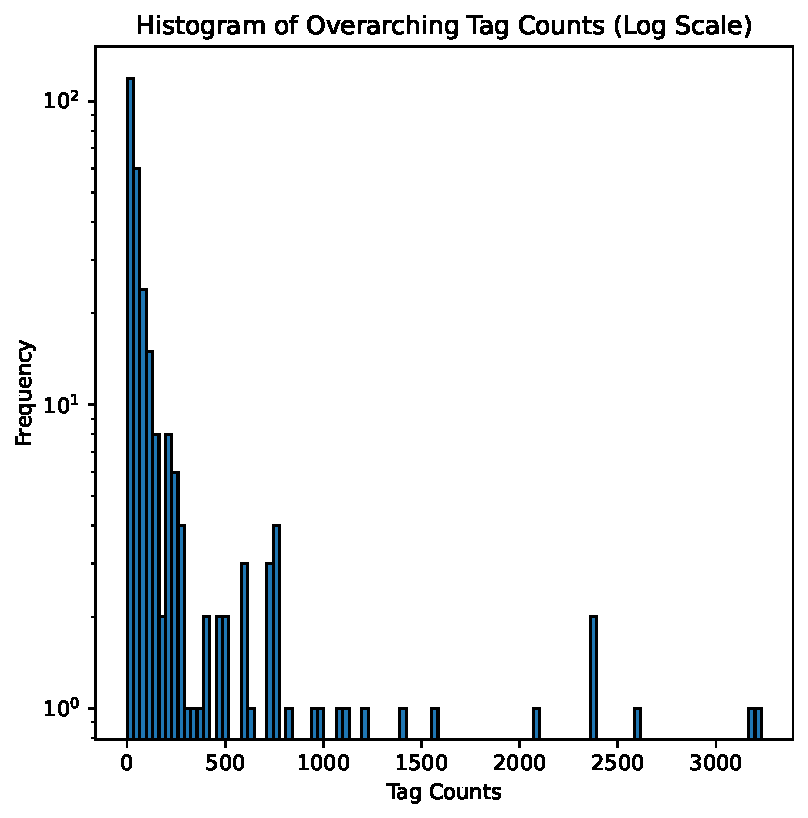
\includegraphics[width=\textwidth]{figures/histogram_overarching_tag_counts_log.pdf}
    \caption{Histogram of overarching tag counts (log scale)}
    \label{fig:histogram_overarching_tag_counts_log}
\end{figure}

We now turn to investigating the tag scores, which are a measure from 0 to 1 that the zeroshot classifier assigns to each tag based on each individual description. \cref{fig:histogram_scores} shows the histogram of tag scores, while \cref{fig:histogram_overarching_scores} shows the histogram of overarching tag scores. We see that the distribution of scores is skewed, with a few tags having a very low score (close to 0) and a few tags having a very high score (close to 1), with the remaining tags having scores in between. This means that the zeroshot classifier is filtering out tags that are not relevant to the descriptions, while assigning high scores to tags that are relevant.

\begin{figure}[h]
    \centering
    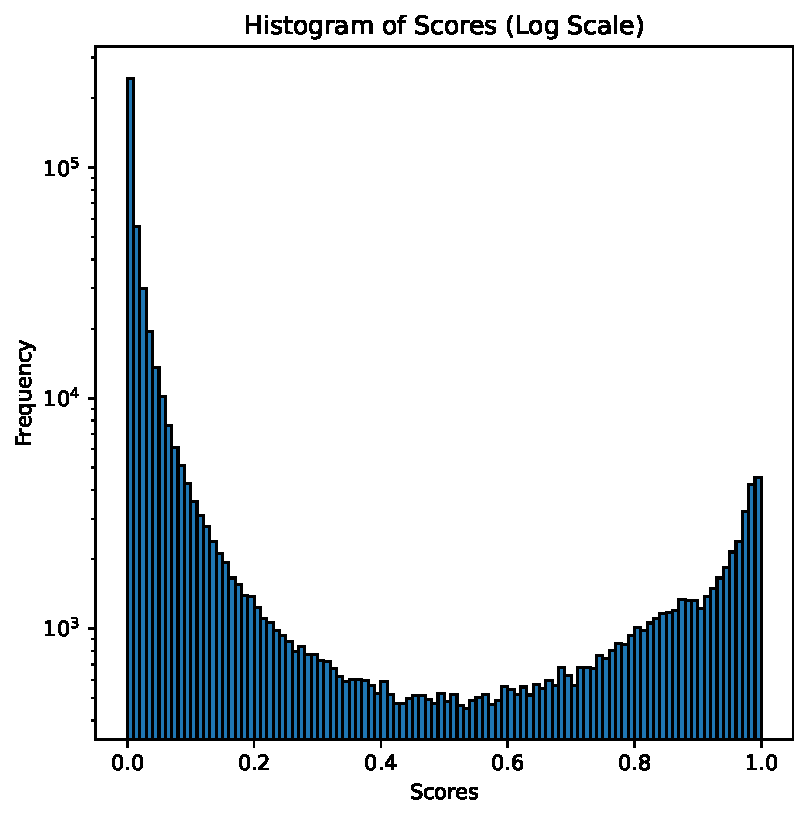
\includegraphics[width=\textwidth]{figures/histogram_scores.pdf}
    \caption{Histogram of tag scores}
    \label{fig:histogram_scores}
\end{figure}

\begin{figure}[h]
    \centering
    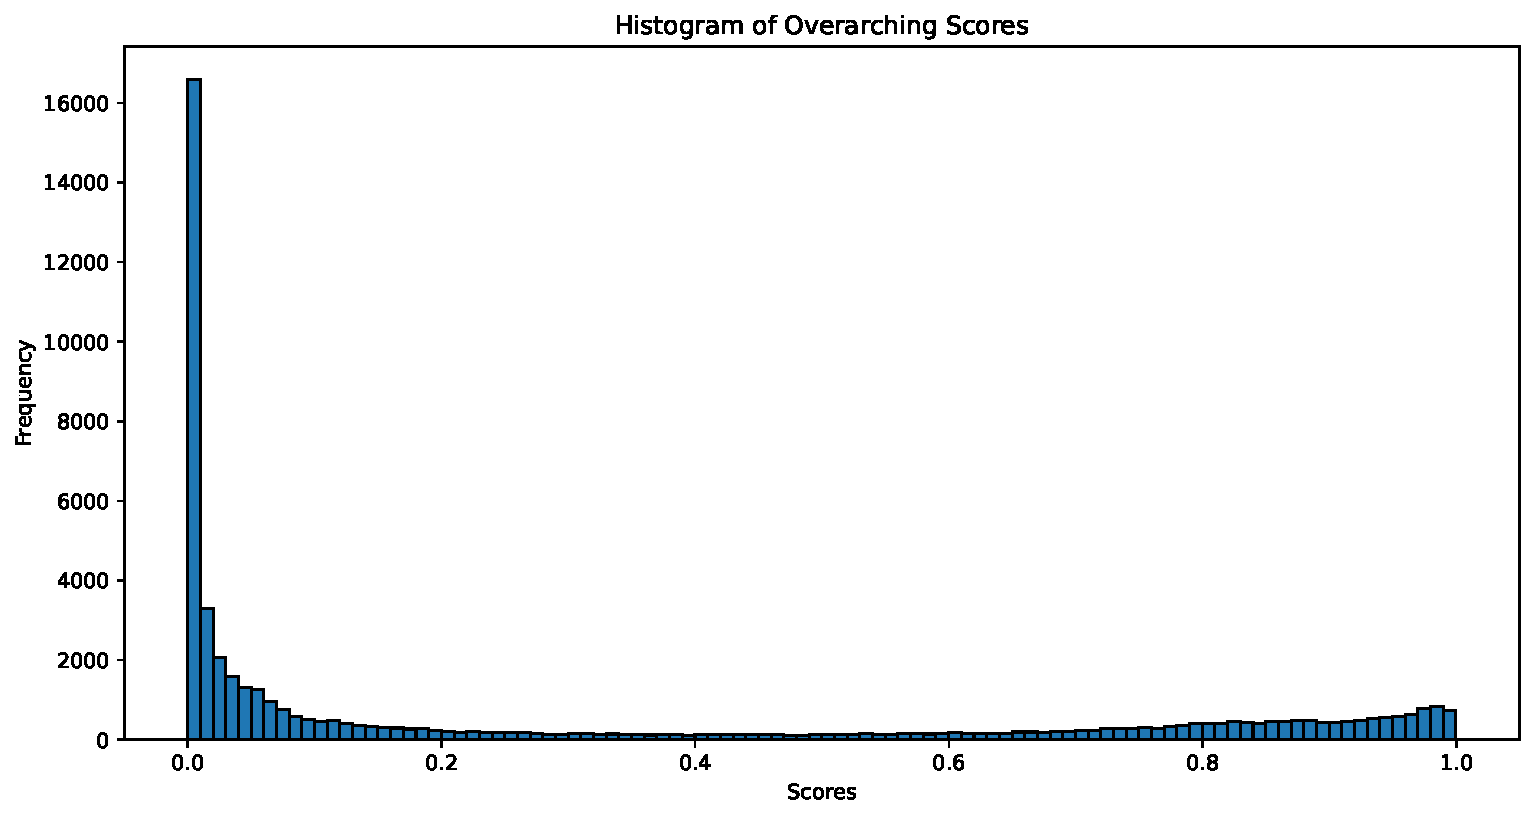
\includegraphics[width=\textwidth]{figures/histogram_overarching_scores.pdf}
    \caption{Histogram of overarching tag scores}
    \label{fig:histogram_overarching_scores}
\end{figure}

\section{Human evaluation}
In this section, we present the results of the human evaluation based on the definition of the study design in \cref{sec:human_evaluation}.

\subsection{Materials}
For the study we design three surveys that follow the structure in \cref{sec:human_evaluation}.

The same dataset descriptions are used across all three surveys to maintain consistency. Based on a pilot study, we select three texts for the \textit{Individual Document Evaluation} stage and two for the \textit{Document Pair Evaluation} stage. The selection criteria focus on appropriate length and complexity to ensure participant comprehension. This number of texts allows participants to complete the survey within approximately 45 minutes, balancing the need for sufficient data collection while preventing participant fatigue.

For brevity, we include only a few examples of the text-tag pairs used in the surveys. All three surveys can be found in the \href{https://github.com/ivangermanov/openml-tags}{GitHub repository} \cite{germanov_topic_modeling_of_2024} under the names of \texttt{proposed\_model\_survey.pdf}, \texttt{baseline\_survey.pdf}, and \texttt{human\_generated\_survey.pdf}.

An example text from the first stage, \textit{Individual Document Evaluation}:

\begin{quote}
    \textbf{FOREX USD/JPY Minute High}

    This dataset contains historical price data of the FOREX USD/JPY from Dukascopy. Each instance, or row, represents one candlestick of one minute. The dataset spans from January first to December thirteenth and does not include weekends, as the FOREX market is not traded on weekends. The timezone of the feature Timestamp is Europe/Amsterdam.
\end{quote}

This text is contained in all three surveys, and for each survey, a different set of tags is provided. \cref{tab:tag_comparison} shows a comparison of tags for different models.

\begin{table}[h]
    \centering
    \begin{tabular}{|>{\raggedright\arraybackslash}p{4cm}|>{\raggedright\arraybackslash}p{4cm}|>{\raggedright\arraybackslash}p{4cm}|}
        \hline
        \textbf{Proposed Model} & \textbf{Human-Generated Survey} & \textbf{Baseline Model} \\ \hline
        Historical Price Data   & Historical Price Data           & Thyrotropin             \\ \hline
        Minute Interval         & Forex                           & Minute                  \\ \hline
        Historical Data         & USD/JPY                         & USD                     \\ \hline
        Forex                   & Currency Pairs                  & Releasing               \\ \hline
        Candlestick             & Yearly Data                     & High                    \\ \hline
        Minute                  & Finance                         & Bid                     \\ \hline
        High                    & Minute High                     & Ask                     \\ \hline
    \end{tabular}
    \caption{Comparison of Tags for Different Models}
    \label{tab:tag_comparison}
\end{table}

For the first task, \textit{Intruder Detection}, an intruder tag, which the participant must identify, is added to the set of tags for each text. The intruder tag is selected at random from the tags of another OpenML dataset.

In the second task, \textit{Tag Quality Assessment}, for each tag, participants are asked to rate the relevance and generality. For each tag set, participants are asked to rate the coverage.

In the second stage, \textit{Document Pair Evaluation}, participants are provided pairs of texts. For example, one pair consists of the following two texts:

\begin{quote}
    \textbf{Movies on Netflix, Prime Video, Hulu, and Disney+}

    This dataset is an amalgamation of data that was scraped, comprising a comprehensive list of movies available on various streaming platforms, and the IMDb dataset, which provides inspiration for analysis.

    Which streaming platform or platforms can I find this movie on? This dataset allows us to explore the availability of movies across different streaming services. Additionally, we can examine the average IMDb rating of movies produced in a specific country, providing insights into the quality of films from different regions.

    \textbf{Popular Movies of IMDb}

    TMDB.org is a crowd-sourced movie information database widely used by various film-related consoles, sites, and apps, such as XBMC, MythTV, and Plex. Dozens of media managers, mobile apps, and social sites utilize its API. At the time of writing, TMDB lists a substantial number of films, which is considerably fewer than IMDb. While not as comprehensive as IMDb, it holds extensive information for most popular and Hollywood films.
\end{quote}

In the first task, \textit{Common Tags Identification}, participants are asked to identify tags that are common to both texts, i.e., the intersection of the two tag sets. For instance, for the two tag sets in \cref{tab:tag_comparison_two_datasets}, the common tags are "Film", "Entertainment", "Movies", and "Media" (as predicted by the model).

\begin{table}[h]
    \centering
    \begin{tabular}{|>{\raggedright\arraybackslash}p{6cm}|>{\raggedright\arraybackslash}p{6cm}|}
        \hline
        \textbf{Movies on Netflix, Prime Video, Hulu, and Disney+} & \textbf{Popular Movies of IMDb} \\ \hline
        Film                                                       & Entertainment                   \\ \hline
        Media                                                      & Technology                      \\ \hline
        Entertainment                                              & Film                            \\ \hline
        Movies                                                     & Media                           \\ \hline
        Film Industry                                              & Movies                          \\ \hline
        Streaming Platforms                                        & Popular Movies                  \\ \hline
                                                                   & Film Information                \\ \hline
    \end{tabular}
    \caption{Comparison of Tags for Two Datasets}
    \label{tab:tag_comparison_two_datasets}
\end{table}


In the second task, \textit{Shared Coverage Assessment}, participants are asked to rate the shared coverage of the tags for both texts.

\subsection{Participants}
Bla bla bla
Bla bla blaBla bla blaBla bla blaBla bla blaBla bla blaBla bla blaBla bla blaBla bla blaBla bla blaBla bla blaBla bla blaBla bla blaBla bla blaBla bla blaBla bla blaBla bla blaBla bla blaBla bla blaBla bla bla


\subsection{Large-scale automated evaluation}
\subsubsection{Automated Intruder Detection}
GPT-4-mini
\subsubsection{Tag Quality Assessment}

\subsubsection{Comparison with Human Evaluation}

% \subsection{Model Robustness}
\subsection{Limitations}

\section{Chapter conclusion}
We answered the research questions for the study, which we defined in methodology, which answers one of the research questions of the thesis (rq4 i believe)